%%%%%%%%%%%%%%%%%%%%%%%%%%%%%%%%%%%%%%%%%
% Journal Article
% LaTeX Template
% Version 1.3 (9/9/13)
%
% This template has been downloaded from:
% http://www.LaTeXTemplates.com
%
% Original author:
% Frits Wenneker (http://www.howtotex.com)
%
% License:
% CC BY-NC-SA 3.0 (http://creativecommons.org/licenses/by-nc-sa/3.0/)
%
%%%%%%%%%%%%%%%%%%%%%%%%%%%%%%%%%%%%%%%%%
%----------------------------------------------------------------------------------------
%       PACKAGES AND OTHER DOCUMENT CONFIGURATIONS
%----------------------------------------------------------------------------------------
\documentclass{article}
\usepackage[francais]{babel} % English language/hyphenation
\usepackage{amsmath,amsfonts,amsthm} % Math packages
\usepackage[utf8]{inputenc}
\usepackage{float}
\usepackage{amsmath}
\usepackage{mathtools}
\usepackage{blindtext}
\usepackage{graphicx} 
\usepackage{caption}
\usepackage[justification=centering]{caption} %centered caption
\usepackage{subcaption}
\usepackage{slashbox}
\usepackage{pict2e}
\usepackage{diagbox}
\usepackage[sc]{mathpazo} % Use the Palatino font
\usepackage[T1]{fontenc} % Use 8-bit encoding that has 256 glyphs
\linespread{1.05} % Line spacing - Palatino needs more space between lines
\usepackage{listings} % insert code

\usepackage{microtype} % Slightly tweak font spacing for aesthetics
\usepackage[hmarginratio=1:1,top=32mm,columnsep=20pt]{geometry} % Document margins
%\usepackage{multicol} % Used for the two-column layout of the document
%\usepackage[hang, small,labelfont=bf,up,textfont=it,up]{caption} % Custom captions under/above floats in tables or figures
%\usepackage{booktabs} % Horizontal rules in tables
\usepackage{float} % Required for tables and figures in the multi-column environment - they need to be placed in specific locations with the [H] (e.g. \begin{table}[H])
\usepackage{hyperref} % For hyperlinks in the PDF
\usepackage{lettrine} % The lettrine is the first enlarged letter at the beginning of the text
\usepackage{paralist} % Used for the compactitem environment which makes bullet points with less space between them
\usepackage{abstract} % Allows abstract customization
\renewcommand{\abstractnamefont}{\normalfont\bfseries} % Set the "Abstract" text to bold
\renewcommand{\abstracttextfont}{\normalfont\small\itshape} % Set the abstract itself to small italic text
\usepackage{titlesec} % Allows customization of titles

%\renewcommand\thesection{\Roman{section}} % Roman numerals for the sections
%\renewcommand\thesubsection{\Roman{subsection}} % Roman numerals for subsections

%\titleformat{\section}[block]{\large\scshape}{\thesection.}{1em}{} % Change the look of the section titles
%\titleformat{\subsection}[block]{\large}{\thesubsection.}{1em}{} % Change the look of the section titles

%\usepackage{pageno}
\usepackage{graphics}% resize tabular
\newcommand\scalemath[2]{\scalebox{#1}{\mbox{\ensuremath{\displaystyle #2}}}} %resize matrix
\usepackage{adjustbox}% resize code lstlisting

\usepackage{fancyhdr} % Headers and footers
\pagestyle{fancy} % All pages have headers and footers
\fancyhead{} % Blank out the default header
\fancyfoot[C]{\thepage} % Blank out the default footer

\fancyhead[C]{Université de Technologie de Compiègne $\bullet$ SY09 $\bullet$ P17} % Custom header text

%----------------------------------------------------------------------------------------
%       TITLE SECTION
%----------------------------------------------------------------------------------------
\title{\vspace{-15mm}\fontsize{24pt}{10pt}\selectfont\textbf{Statistique descriptive,\\Analyse en composantes principales}} % Article title
\author{
\large
{\textsc{Yanqing ZENG~ GI05}}\\
{\textsc{Minh Tri LÊ GI02}}
}


%----------------------------------------------------------------------------------------
\begin{document}
\maketitle % Insert title
\thispagestyle{fancy} % All pages have headers and footers


\section*{Introduction}
Le but de ce premier TP est d'une part de décrire puis découvrir des relations au sein de ces données en appliquant des concepts élémentaires de statistique.
D'autre part, l'objectif est de réaliser une analyse en composantes principales (ACP) afin d'identifier des similarités ou différences dans les données et de représenter les données dans une dimension réduite sans trop perdre d'information. % Intro ACP à compléter...

\section{Statistique descriptive}


\subsection{Notes}
Ce jeu de données comprend les notes de 296 étudiants ayant suivi SY02 au semestre P16. Il comporte 11 variables dont 3 quantitatives et 8 qualitatives.


\subsubsection*{1.}\label{1.1.1}

% Tableau résumé
\begin{table}[!ht]
\caption{Résumé des variables du jeu de données \textit{Notes}}\label{table1.1}
\label{Table1}
\centering
\resizebox{11cm}{!}{
\begin{tabular}{|l|c|c|c|}
\hline
 & Nature & Domaine de définition & Nombre de valeurs \textit{NA} \\
\hline
Nom & Qualitative & Etu\textit{i}, \textit{i} $\in$ $\lbrack1;296\rbrack$ ($\mathbb{N}$)& 0 \\
\hline
Specialite & Qualitative & $\lbrace$TC,HuTech, ISS, GB,& 0 \\
& & GI,GSU,GM,GSM,GP$\rbrace$&\\
\hline
Niveau & Qualitative &$\lbrack1;6\rbrack$ ($\mathbb{N}$)& 0 \\
\hline
Statut & Qualitative & $\lbrace$UTC, Echange$\rbrace$  & 0 \\
\hline
Dernier diplôme& Qualitative & $\lbrace$BAC, DUT, AUTRE $1^{er}$cycle, CPGE, BTS,& 6 \\
obtenu& &DEUG, LICENCE,&\\
& &INGENIEUR, ETRANGER SUPERIEUR,&\\
& & ETRANGER SECONDAIRE, &\\
& & AUTRE DIPLOME SUPERIEUR &\\
& &AUTRE 2E cycle$\rbrack$ &\\
\hline
Note median & Quantitative &$\lbrack0;20\rbrack$ ($\mathbb{R}$) & 3 \\
\hline
Correcteur median & Qualitative & Cor\textit{i}, \textit{i} $\in$ $\lbrack1;8\rbrack$ ($\mathbb{N}$)& 3\\
\hline
Note final & Quantitative & $\lbrack0;20\rbrack$ ($\mathbb{R}$)& 12\\
\hline
Correcteur final & Qualitative& Cor\textit{i}, \textit{i} $\in$ $\lbrack1;8\rbrack$ ($\mathbb{N}$)& 12\\
\hline
Note totale & Quantitative & $\lbrack0;20\rbrack$ ($\mathbb{R}$) & 12 \\
\hline
Resultat & Qualitative ordinale& $\lbrack$A,B,..., F, FX$\rbrack$& 12 \\
\hline
\end{tabular}
}

\end{table}
% Fin tableau résumé

Le tableau \lbrack\ref{table1.1}\rbrack indique une liaison entre les variables \textit{Note median} et \textit{Correcteur median} ainsi que \textit{Note final, Correcteur final, Note totale et Resultat}.
On en déduit que si un étudiant n'a pas eu de note au médian (\textit{resp. final}) (pour cause d'absence) alors aucun correcteur du médian (\textit{resp. final}) n'a pu corrigé sa copie. De plus, si un correcteur n'a pas pu corrigé le final alors l'étudiant n'a pas de \textit{note totale} et de \textit{resultat}.

Les 6 valeurs manquantes de \textit{dernier diplome obtenu} correspondent aux 6 étudiants en échange. De plus, on observe que ces 6 étudiants n'ont pas obtenu SY02 ou ont été absents.

Un résumé des statistiques des valeurs quantitatives est en table \lbrack\ref{anx1}\rbrack.
%Annexe : résumé moyenne, écart type,...

\subsubsection*{2.} 

Nous recherchons d'abord quelles variables influencent la note totale et par équivalence, la réussite à l'UV.

Les box plot \lbrack\ref{anx2}\rbrack montrent une disparité de la note totale en fonction de la spécialité/niveau et du dernier diplôme obtenu.
Au sein d'une même specialité (une même couleur) mais d'un niveau différent, la réussite n'est pas homogène, de même entre les différentes spécialités. 
Les GSU/TC semblent le mieux réussir contrairement aux GP/GSM/HuTech, cependant il faut noter que les GP, TC et HuTech ne représentent qu'une petite partie des indivus (respectivement 5.4\%, 3.7\% et 0.3\%) donc ce n'est pas très représentatif.
Il y a aussi quelques valeurs aberrantes, pour les GI et GSU par exemple.\\
Nous avons effectué des tests du Chi2 pour la spécialité et le niveau (table \lbrack\ref{anx6}\rbrack). On rejette donc l'hypothèse d'indépendance entre la specialite et le niveau.

Concernant la variable \textit{dernier diplome obtenu}, les CPGE ont le plus de disparités (Étendue = 15.8 soit 79\% de 20). Ceux issus de "etranger secondaire" semblent le mieux réussir suivi de BAC et Licence. 
Némanmoins, il faut savoir que les licences et etranger secondaire ne sont pas quantitativement bien représentés (respectivement 3.1\% et 1.7\% de la part des individus). Il y a encore quelques valeurs aberrantes pour ceux issus du BAC. Le test du Chi2 (table \lbrack\ref{anx6}\rbrack) ne rejette pas l'hypothèse d'indépendance pour le dernier diplome obtenu.



\begin{figure}[H] % Boxplot specialite & niveau ; diplome ~ res 

\centering
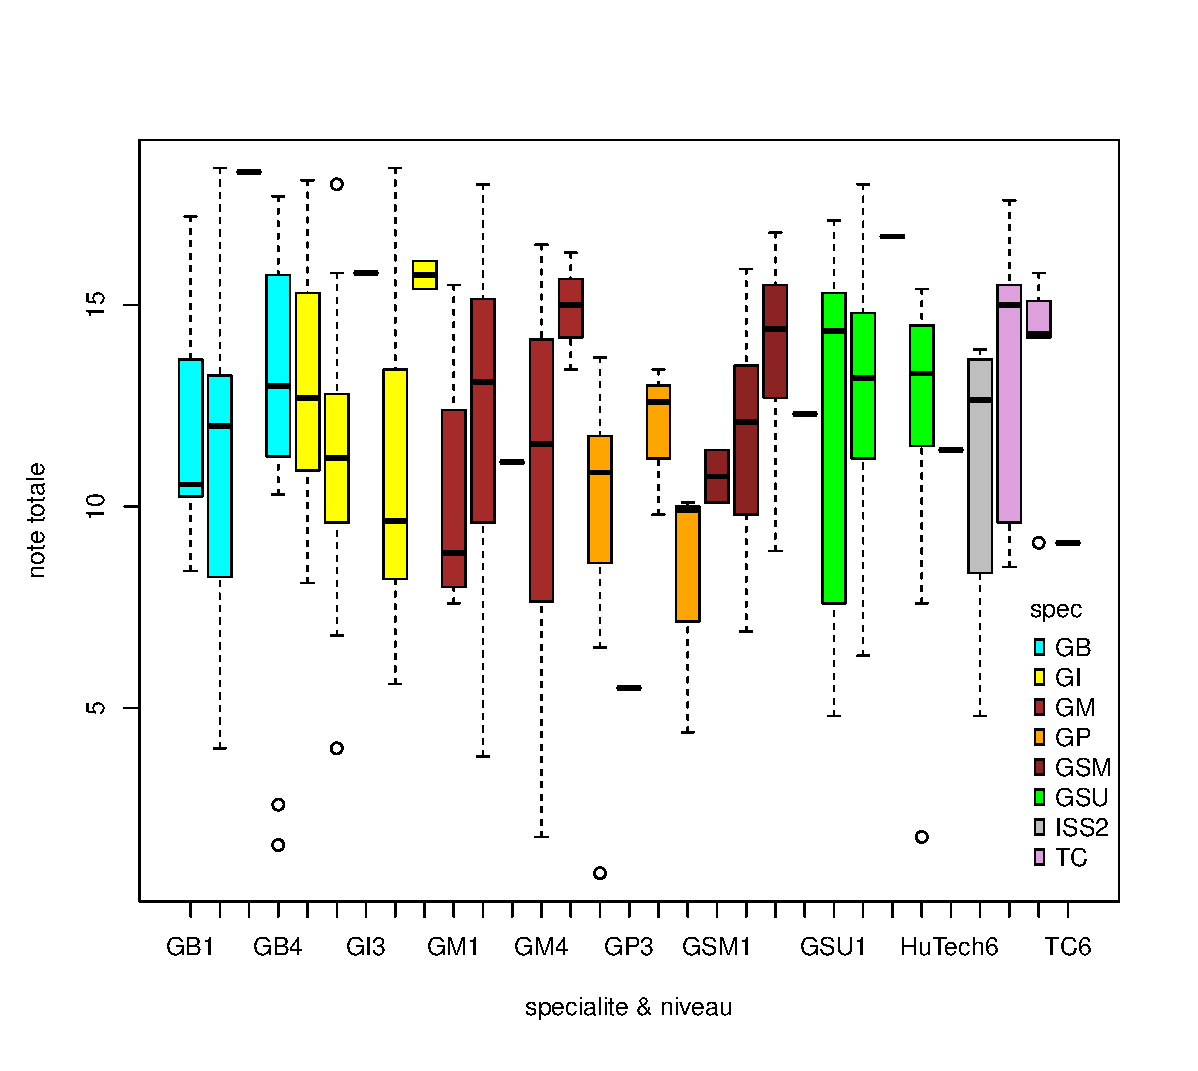
\includegraphics[scale=0.36]{./img/boxplot_spec_niv_res.eps}
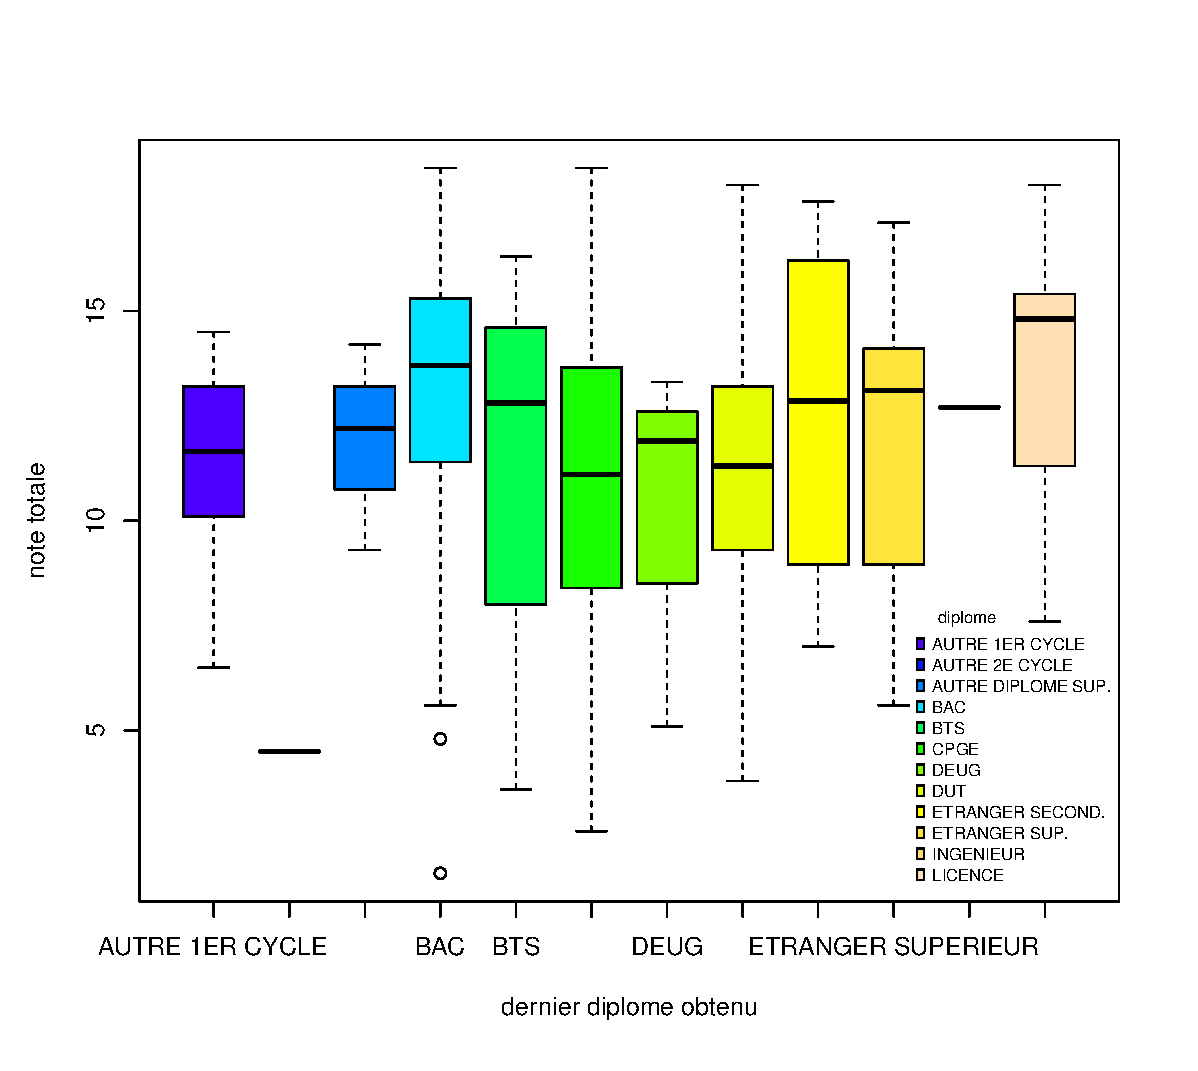
\includegraphics[scale=0.36]{./img/boxplot_dipl_res.eps}
\caption{Box plot de la \textit{note totale} en fonction de la \textit{specialite et du niveau} ainsi que du \textit{dernier diplôme obtenu}}
\label{anx2}
\end{figure}

Le premier box plot de la figure \lbrack\ref{anx3}\rbrack confirme le fait que les étudiants en échange ne réussissent pas l'UV.\\
Il y a un peu d'hétérogénéité entre les notes données par les correcteurs median, mais cela est plus marqué pour la note finale ; ce qui se répercute sur la note totale car le dernier box plot ressemble au box plot du correcteur final.
\begin{figure}[!ht]
\begin{center}
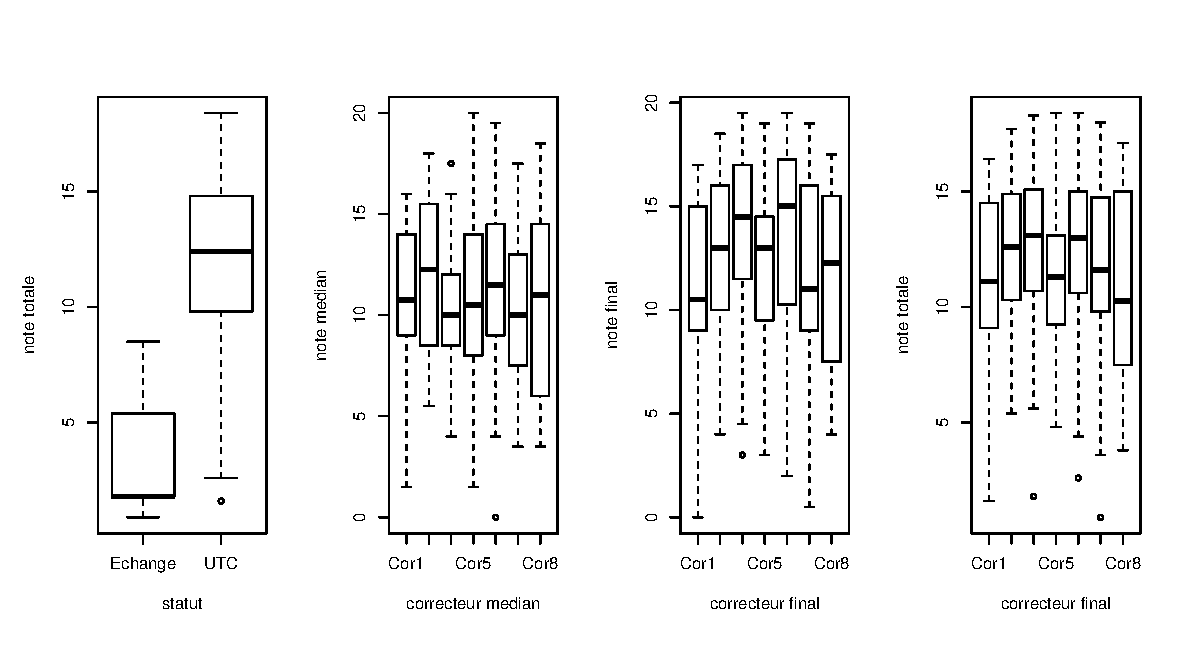
\includegraphics[scale=0.52]{./img/boxplot_par_1-3_2.eps}
\caption{Box plot des notes en fonction du \textit{statut} et du \textit{correcteur}}
\label{anx3}
\end{center}
\end{figure}

Pour tester si un correcteur influence la note obtenue, nous avons effectué des tests de Student (table \ref{anx7}). Pour l'examen médian, il ne semble pas y avoir de dépendance entre les correcteurs. En revanche, pour les correcteurs [1,4], [1,6] de l'examen final, l'hypothèse d'indépendance est rejetée : certains correcteurs influencent la note obtenue.



L'intersection des droites moyennes du graphique \lbrack\ref{anx4}\rbrack n'est pas au centre, mais plutôt décalé vers le haut et un peu à droite. Cela indique une meilleure note au final qu'au médian et une réussite générale des étudiants. Il y a une concentration des points dans la partie haute à droite. Ces étudiants ont eu une note au-dessus de la moyenne au médian ou au final ou peut être les deux. À l'inverse, moins d'étudiants ont eu une mauvaise note au médian ou une mauvaise note au final ou peut être les deux.
\begin{figure}[H] % Scatterplot note median ~ note final
\begin{center}
\includegraphics[scale=0.40]{./img/scatterplot_median_final_avg-bar.png}
\caption{Scatter plot de la \textit{note median} et de la \textit{note final}}
\label{anx4}
\end{center}
\end{figure}
Le tableau de corrélation \lbrack\ref{anx5}\rbrack révèle en fait une corrélation plutôt faible (0.386) entre \textit{note median} et \textit{note final} donc il y a peu de lien entre les étudiants ayant eu une bonne note au médian et au final. La forte corrélation entre \textit{note total} et \textit{note final} (0.912) (resp. \textit{note median} : 0.730) est expliquée par la notation suivante : $\textit{note total} = 0.4*\textit{note median}+0.6*\textit{note final}$.\\
Ainsi, la réussite ou l'échec au médian n'est pas déterminante de la note finale, mais ces dernières le sont pour la réussite globale.




%%%%%%%%%%%%%%%%%%%%% FIN NOTES

%\newpage % figure désordonnée...

%%%%%%%%%%%%%%%%%% CRABS
\subsection{Données crabs}
Ce jeu de données comprend 200 enregistrements de données sur des crabes. Il comporte 2 variables qualitatives et 5 variables quantitatives. La colonne 'index' est inutile pour cette analyse.
Il n'y a aucune valeur \textit{NA} et deux espèces de crabe 'B' (bleu) et 'O' (orange). Un résumé des statistiques des variables quantitatives est en table \ref{anx2.1}.

\subsubsection*{1.}\label{1.2.1}

% Supprimé car déjà mentionné dans la question et dit juste au dessus.

% %table  résumé - crabs
% \begin{table}[!ht]
% \caption{Résumé des variables du jeu de données  \textit{Crabs}}\label{table1.2}
% \label{Table2}
% \centering
% \resizebox{6.5cm}{!}{
% \begin{tabular}{|l|c|c|}

% \hline
%  & Nature & Domaine de définition\\
% \hline
% sp (species) & Qualitative & $\lbrace$B, O$\rbrace$\\
% \hline
% sex & Qualitative & $\lbrace$M, F$\rbrace$\\
% \hline
% FL (Frontal Lobe)  & Quantitative & $\mathbb{R}$ en mm\\
% \hline
% RW (Rear width) & Quantitative & $\mathbb{R}$ en mm\\
% \hline
% CL (Carapace length) & Quantitative & $\mathbb{R}$ en mm\\
% \hline
% CW (Carapace width) & Quantitative & $\mathbb{R}$ en mm\\
% \hline
% BD (Body depth) & Quantitative & $\mathbb{R}$ en mm\\
% \hline

% \end{tabular}
% }
% \end{table}

Le diagramme en boîte \lbrack\ref{fig:sp_sex_morphologique}\rbrack nous montre les relations entre la morphologie et les caractéristiques qualitatives (l'espèce et le sexe). Cela nous donne l'intuition que ces caractéristiques et la morphologie ne sont pas indépendantes. Afin de vérifier la dépendance, nous effectuons un test de Student (Table \lbrack\ref{Table2.1}\rbrack).

\begin{figure}[!ht]
\centering
\includegraphics[width=8.7cm]{./img/box_plot_sex.png}% nom d'image inversé avec 'sp' car il y a 'B', 'O' en légende
\includegraphics[width=8.7cm]{./img/box_plot_sp.png}
\caption{Box plot de la morphologie en fonction de l'espèce (gauche) et du sexe (droite)}
\label{fig:sp_sex_morphologique}
\end{figure}

Le diagramme \lbrack\ref{fig:sp_sex_morphologique}\rbrack nous montre que la distribution des caractéristiques morphologiques de l'espèce 'O' est généralement plus grande que l'espèce 'B', en particulier pour le caractère 'FL' et 'BD'. Cela peut être expliqué par le fait que 'FL' et 'BD' ont les p-values les plus significatives pour le test de Student (Table \ref{Table2.1}) avec l'espèce.\\
Les diagrammes en boîte \lbrack\ref{fig:sp_sex_morphologique}\rbrack nous montre que la distribution de toutes les variables quantitatives en fonction du sexe est similaire sauf pour le caractère 'RW'. L'individu femelle a à priori un plus grand 'RW' que l'individu mâle. La figure \ref{fig:pairs-plot_identif_sex} montre que le sexe peut être déterminé en grande partie à partir de 'RW' mais aussi [RW, FL], [RW, CL], [RW,BD] et [RW, CW].
Cela est confirmé par la p-value du test de Student entre le sexe et les variables quantitatives (Table \ref{Table2.1}) : l'hypothèse d'indépendance est rejetée.
\begin{figure}[!ht]
\centering
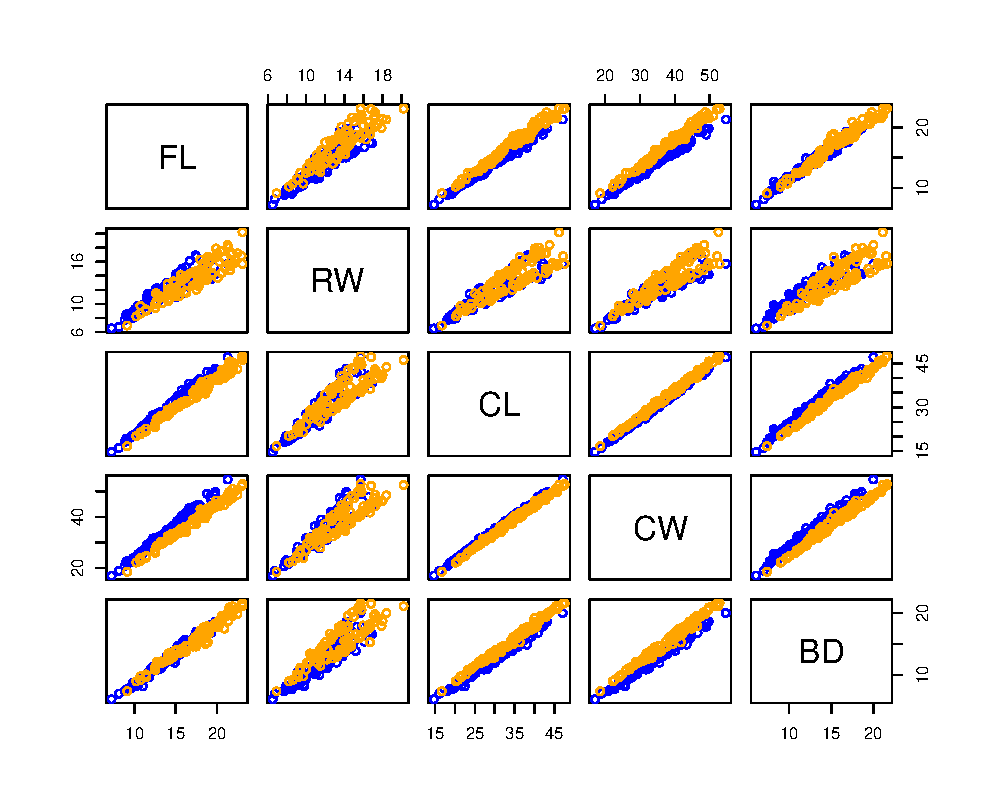
\includegraphics[width=5.7cm]{./img/1-2-pairs-plot_sp.eps}
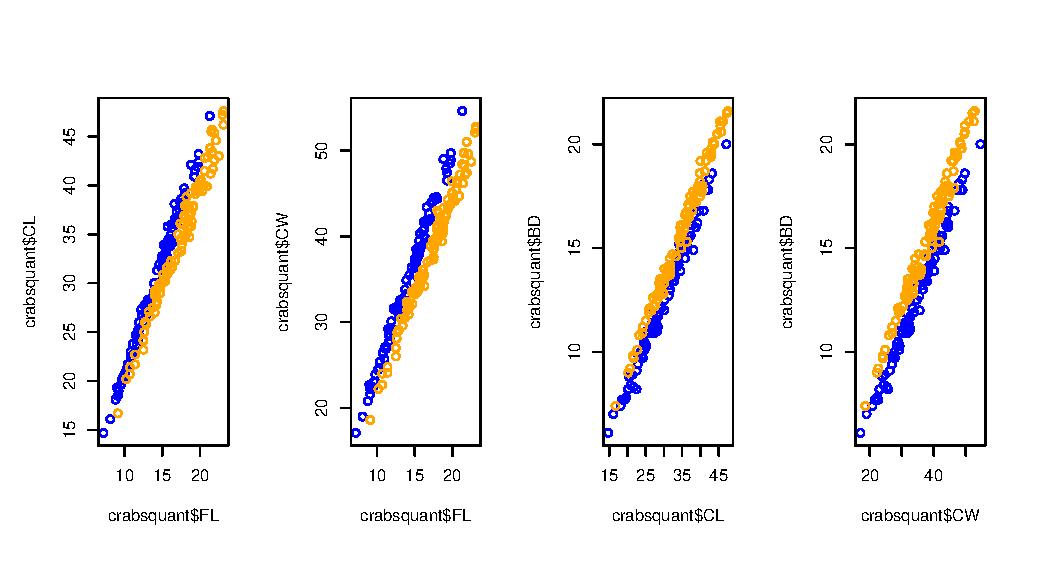
\includegraphics[width=9cm]{./img/1-2-pairs_identif_sp.eps}
\caption{Représentation des individus en fonction de l'espèce ('O' : Orange, 'B' : Bleu) par les variables quantitatives}
\label{fig:pairs-plot_sp}
\end{figure}

%TO SUPPRIMER OU METTRE DANS ANNEXS?
% j'ai resize, donc ça va je pense ?

% \begin{figure}[!ht]
% \centering
% 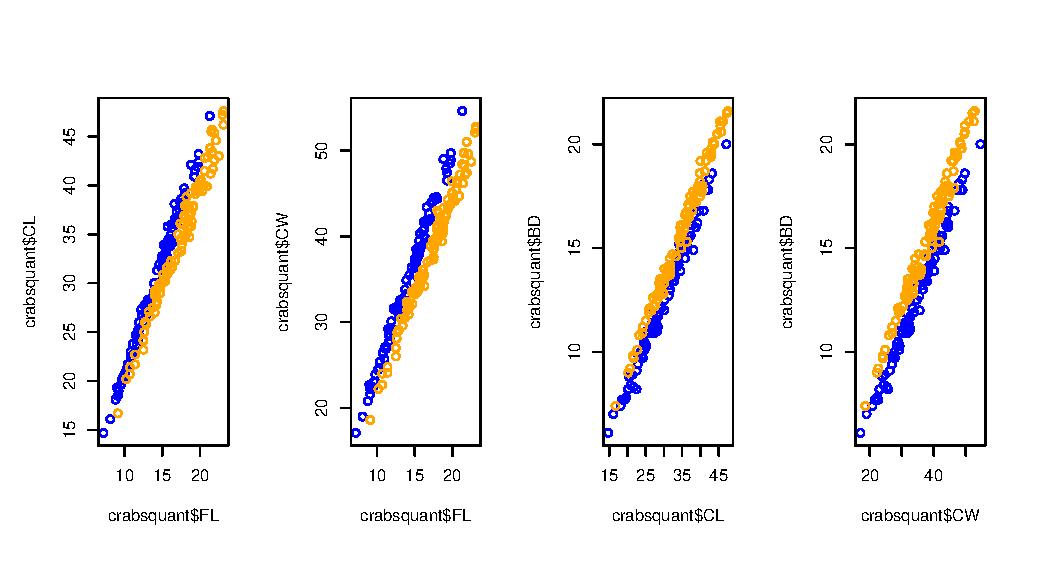
\includegraphics[width=9cm]{./img/1-2-pairs_identif_sp.eps}
% \caption{Représentation des individus en fonction de l'espèce ('O' : Orange, 'B' : Bleu) par les variables quantitatives identifiants fortement l'espèce}
% \label{fig:pairs-plot_identif_sp}
% \end{figure}

La figure \ref{fig:pairs-plot_sp} montre qu'il est possible d'identifier l'espèce en très grande partie avec les variables [FL,CL] et donc [FL,CW] car CL et CW sont très corrélées (voir table \ref{table1.2.2}) De même pour [BD,CW] et donc [BD,CL]. Il y a un recouvrement très faible entre les deux espèces.


% \begin{figure}[!h]
% \centering
% \includegraphics[width=8.4cm]{./img/box_plot_sp.png}
% \caption{Diagramme en boîte de la morphologie en fonction du sexe ('F' : rouge, 'M' : bleu)}
% \label{fig:sp_ssp_morphologique}
% \end{figure}

%TO SUPPRIMER OU METTRE DANS ANNEXS?
% => Annexe
 
% La figure \lbrack\ref{fig:sp_sex_ssp_morphologique}\rbrack nous montre que les femelles de l'espèce 'O' sont généralement plus grandes que les tous les autres crabes alors que les femelles de l'espèce 'B' sont généralement les plus petites.
% Cela nous permet à priori d'identifier une majorité de crabe femelle de l'espèce 'O' et 'B' en sachant la variable 'FL'.
%TO SUPPRIMER ?
% OK

% \begin{figure}[!ht]
% \centering
% \includegraphics[width=5.7cm]{./img/1-2-pairs-plot_sex.eps}
% \caption{Représentation des individus en fonction du sexe ('F' : rouge, 'M' : Bleu) par les variables quantitatives}
% \label{fig:pairs-plot_sex}
% \end{figure}

%table p valeur 
%table  résumé - crabs


%Nous en déduisons qu'il est possible d'identifier l'espèce à partir de n'importe quelle variable morphologique. Les p-value du sexe (Table \ref{Table2.1}) nous montre que le sexe est dépendant de la variable RW. 
%mais la distribution  par le diagramme en boîte semble proche. Par conséquence, il exite un haut taux d'erreurs.
% => Pas totalement d'accord : La médiane du sexe F est au dessus du 1er quartile du sexe M <=> La moitié des F est plus grande qu'un quart des M ==> Il n'y a pas indépendance avec RW à mon avis. Pour les autres variables, c'est bien homogène oui.



\subsubsection*{2.}\label{1.2.2}

% \begin{figure}[!ht]
% \centering
% \includegraphics[width=7cm]{./img/1-2-pairs-plot_neutral.eps}
% \caption{Représentation des individus par les variables quantitatives}
% \label{fig:pairs-plot_neutr}
% \end{figure}
La représentation par les paires de variables (Figure \ref{fig:pairs-plot_sp}) nous montre que les 5 variables quantitatives ont une forte corrélation linéaire. Les valeurs de corrélation sont présentées dans la table \lbrack\ref{table1.2.2}\rbrack. La matrice de corrélation montre bien la forte relation linéaire entre les variables, la plus petite valeur est 0.889 ('RW', 'BD'), ce qui est très élevé.\\
Nous pouvons interpréter cela par le fait que ces variables sont des mensurations de crabes, donc chaque partie du corps d'un crabe est proportionnelle aux autres. 'CL' (Carapace length) et 'CW' (Carapace width) sont corrélées à 0.995 car la longueur et la largeur de la carapace sont proportionnelles.
%Par contre, la corrélation ne indique pas  une variable est la cause de l'autre. 

En conséquence, les individus représentés par ces variables se recouvrent. Il est donc difficile de discerner correctement des groupes en travaillant sur 5 dimensions fortement corrélées.\\ Pour s'affranchir de ce phénomène, on peut appliquer une analyse en composantes principales (ACP) et réduire les dimensions. On obtient alors des combinaisons linéaires indépendantes des variables, ce qui permet alors de visualiser les individus dans une nouvelle représentation. En observant la figure, il semble qu'une seule dimension peut déjà exprimer une partie de l'information.


%pima
\subsection{Données pima}
\subsubsection*{1.}\label{1.3.1}
Ce jeu de données comprend 532 individus de sexe féminin décrit par huit variables. Il comporte 7 variables quantitatives et 1 variable qualitative.

Un résumé des statistiques des variables quantitatives est en annexe [\ref{anx3.1}]

\subsubsection*{2.}\label{1.3.2}

La figure \ref{fig:pima-quant_plot} montre que les individus sont très dispersés entre eux selon les variables quantitatives.
La table \ref{table1.3.1} confirme que les variables sont peu corrélées entre elles sauf pour npreg et age (0.641), bmi et skin (0.647). Autrement, les valeurs sont inférieures à 0.350. Il y a donc beaucoup de recouvrement sur la représentation des individus diabétiques et non-diabétiques.

\begin{figure}[!ht]
\centering
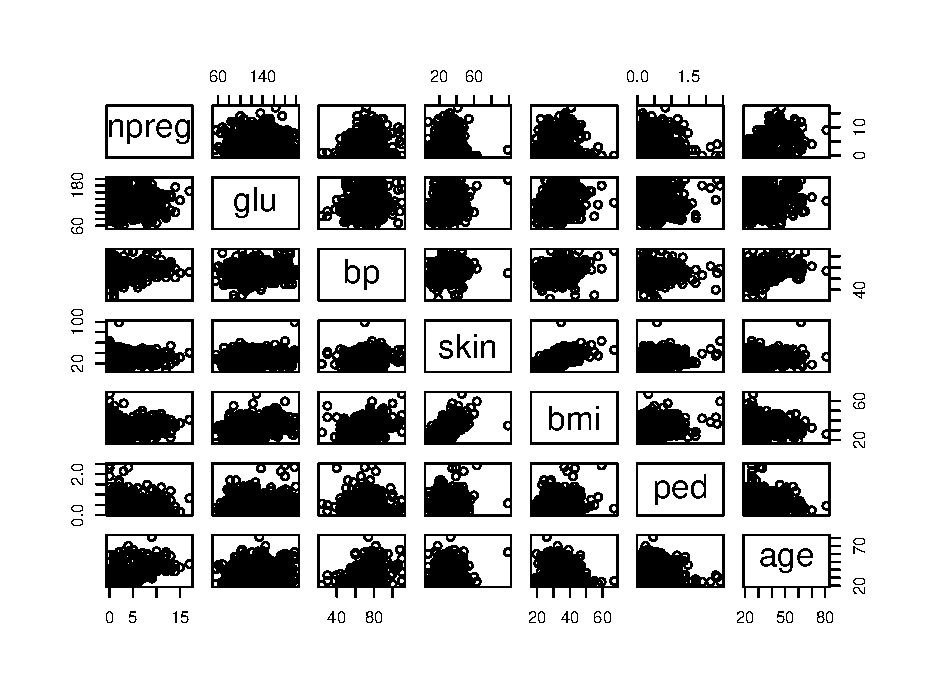
\includegraphics[width=7cm]{./img/pima-quant_plot.eps}
\caption{Représentation des individus par les variables quantitatives de \ref{1.3.1}}
\label{fig:pima-quant_plot}
\end{figure}



\begin{figure}[H]
\centering
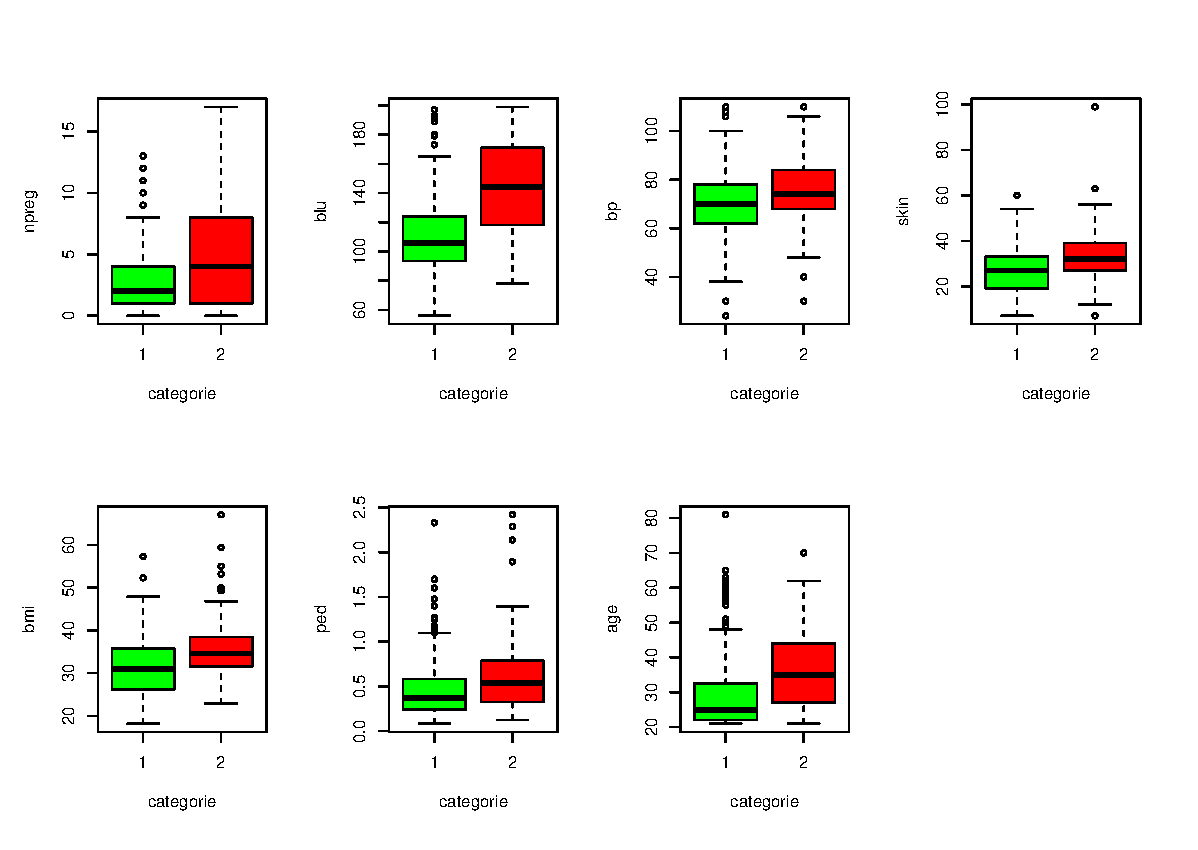
\includegraphics[width=10.71cm]{./img/pima_boxplot.eps}
\caption{Diagramme en boîte des données pima en fonction du diabète\\(Diabétique en rouge, non-diabétique en vert)}
\label{fig:pima_boxplot}
\end{figure}

La figure \ref{fig:pima_boxplot} nous montre qu'il y a des valeurs aberrantes dans ce jeu de données, en particulier pour l'âge des non-diabétiques. Les individus diabétiques semblent avoir les valeurs les plus élevées par rapport aux non-diabétiques pour tous les indicateurs, surtout pour le glucose.\\ Pour vérifier l'influence du facteur "diabète", nous avons testé l'hypothèse d'indépendance par le test de Student (table \ref{table1.3_student})

D'après les résultats du test, on rejette l'hypothèse $H_{0}$ : \textit{Les indicateurs sont indépendants de la variable diabète.} Autrement dit, le diabète influence bien les variables quantitatives. La p-value de la variable glu est très significative, cela confirme que le diabète a bien une forte influence sur le taux plasmatique de glucose, ce qui est cohérent (pour le diabète).

Ainsi, il va être difficile de discerner les diabétiques des non-diabétiques en réduisant le nombre de variables avec l'ACP car le diabète influence toutes les variables. De plus, les variables sont en général peu corrélées entre elles donc il n'existe peut-être pas de combinaisons linéaire indépendante avec moins de composantes qu'actuellement.

\section{Analyse en composantes principales}

%ACP théorique
\subsection{Exercice théorique}
\label{2.}
\subsubsection*{1.}
Les individus Cor2, Cor3 sont d'abord enlevés car ils ont des valeurs NA.\\
Après avoir centré les données par colonne, on obtient la matrice X qui prend comme variable : \textit{moy.median, std.median, moy.final, std.final} et les individus \textit{Cor1, Cor4, Cor5, Cor6, Cor7, Cor8} :
\begin{equation} 
X=
\left(   
\scalemath{0.70}{
  \begin{array}{cccc}   
    -0.0058 & -0.1556 & -1.2133  &0.0679\\  
    -0.4795 &-1.0130 &1.2815       & -0.1723\\  
     0.2654 & 0.3572 &-0.3235& -0.5436\\
      0.7858 &0.2473  &1.2616  &0.3617\\
      -0.5917 &-0.0257 &-0.2490 &-0.0705\\
      0.0258  &0.5898 &-0.7574  &0.3568\\
    
  \end{array}
  }
\right)                 
\end{equation}

La matrice de la variance V:
\begin{equation}
V=\frac{1}{n}X^{T}X=
\left( 	
\scalemath{0.75}{
	\begin{array}{cccc} 
	0.2114&  0.1343&  0.0710& 0.0455\\
    0.1344&  0.2646& -0.2255& 0.0453\\
    0.0710& -0.2255&  0.9077& 0.0127\\
    0.0455&  0.0453&  0.0127& 0.0988\\
    \end{array}
    }
\right)
\label{mat_V}
\end{equation}

En diagonalisant la matrice (\ref{mat_V}), on obtient les valeurs et vecteurs propres de la matrice V :
\begin{center}
$\lambda_{1}=0.97994449,\lambda_{2}=0.36748816,\lambda{3}=0.08318286,\lambda_{4}=0.05200103$

\end{center}

La matrice des vecteurs propres U et donc les axes factoriels :
\begin{equation}
U=
\left(
\scalemath{0.75}{
	\begin{array}{cccc} 
    -0.0368& 0.7043& -0.2332&  0.6695\\
    0.2942& 0.6469& -0.0943& -0.6972\\
    -0.9550& 0.1720& -0.0206& -0.2406\\
    -0.0006& 0.2364&  0.9676&  0.0883\\
    \end{array}
    }
\right) 
\end{equation}

Les pourcentages d'inertie expliquée par chacun des axes factoriels : $E_{k}=\frac{\lambda_{1}+\lambda_{2}+...\lambda_{k}}{\sum_{\alpha=1}^{p}\lambda_{\alpha}}*100$ :
% \[
% E_{1}=0.6609561=66.1\% 
% \]
% \[
% E_{2}=0.9088207=90.09\%
% \]
% \[
% E_{3}=0.9649262=96.5\%
% \]
% \[
% E_{4}=1.00000=100\%
% \]

\begin{table}[!h]
\centering
\caption{Inertie expliquée par les axes factoriels}
\label{Table3.1}
\resizebox{8.4cm}{!}{%
\begin{tabular}{l|c|c|c|c}
& k=1 & k=2 & k=3 & k=4\\
\hline
%Valeur  &0.97994449&0.36748816&0.08318286&0.05200103\\
Inertie expliquée (\%) &66.1\% & 24.8\% & 5.61\% & 3.51\%\\
Inertie expliquée cumulée (\%) ($E_{k}$) & 66.1\% & 90.09\% & 96.5\% & 100\%\\

\end{tabular}
}

\label{2.1.tab_inertie}
\end{table}

La table \ref{2.1.tab_inertie} montre que les deux premiers axes factoriels contiennent une grande partie de l'inertie expliquée (90\%).

\subsubsection*{2.}
La matrice des composantes principales et donc les coordonnées des individus dans le nouvel espace représenté par la figure \ref{q.1.premier_plan_fac} :
\begin{equation}
C=XU=
\left(
\scalemath{0.75}{
	\begin{array}{cccc}
    1.1131& -0.2973&  0.1068&  0.4025\\
    -1.5042& -0.8134&  0.0142&  0.0617\\
    0.4045&  0.2338& -0.6149& -0.0415\\
    -1.1613&  1.0159&  0.1174&  0.0820\\
    0.2521& -0.4929&  0.0773& -0.3245\\
    0.8957&  0.3538&  0.2993& -0.1801\\
    \end{array}
}    
\right) 
\end{equation}

\begin{figure}[H]
\centering
\includegraphics[width=5.6cm]{./img/acp_premier_plan.png}
\caption{Représentation des six individus dans le premier plan factoriel}
\label{q.1.premier_plan_fac}
\end{figure}
%TO DO  inserer figure du premier plan


\subsubsection*{3.}
La matrice de coordonnées des variables dans le nouvel espace :

\begin{table}[!ht]
\centering
\caption{Coordonnées des variables dans le nouvel espace}
\label{Table2.1.3}
\resizebox{6.8cm}{!}{%
\begin{tabular}{c|cccc}
&Comp.1&Comp.2&Comp.3&Comp.4\\
\hline
moy.median& -0.079 &0.928& -0.146 & 0.332\\
std.median & 0.566& 0.762& -0.053 &-0.309\\
moy.final&  -0.992 &0.109& -0.006& -0.058\\
std.final & -0.002 &0.456&  0.888 & 0.064\\

\end{tabular}
}
\end{table}

D'après la matrice de coordonnées, on peut déduire que la première composant exprime une majorité de l'information de la variable moy.final, et la deuxième composante exprime bien la variable moy.median et un peu moins std.median.
La troisième composante explique uniquement bien la variable std.final.

Plus une variable s'éloigne d'un axe, plus elle est expliquée par celui-ci.

\begin{figure}[H]
\centering
\includegraphics[width=7.5cm]{./img/cercle_1.png}
\caption{Représentation des 4 variables dans le premier plan factoriel}
\label{2.1.var_plot_fac}
\end{figure}
%TO  DO
\subsubsection*{4.}
%TO DO
Quand k=1 :
\[
\sum_{\alpha=1}^{1}c_{\alpha}u_{\alpha}{'}=
\left(
\scalemath{0.75}{
	\begin{array}{cccc}
    -0.0410&  0.3275& -1.0631& -0.0006\\
    0.0554& -0.4425&  1.4365&  0.0009\\
    -0.0142&  0.1190& -0.3864& -0.0002\\
    0.0428& -0.3416&  1.1091&  0.0007\\
    -0.0093&  0.0742&-0.2407& -0.0001\\
    -0.0330&  0.2635& -0.8554& -0.0005\\
    \end{array}
    }
\right)   
\]

Quand k=2 :
\[
\sum_{\alpha=1}^{2}c_{\alpha}u_{\alpha}{'}=
\left(
\scalemath{0.75}{
	\begin{array}{cccc}
    -0.2504&  0.1351& -1.1142& -0.0709\\
    -0.5175& -0.9687&  1.2967& -0.1915\\
    0.1498&  0.2703& -0.3461&  0.0551\\
    0.7583&  0.3156&  1.2838&  0.2409\\
    -0.3564& -0.2447& -0.3255& -0.1167\\
    0.2162&  0.4924& -0.7946&  0.0832\\
    \end{array}
    }
\right)   
\]

Quand k=3 :
\[
\sum_{\alpha=1}^{3}c_{\alpha}u_{\alpha}{'}=
\left(
\scalemath{0.75}{
	\begin{array}{cccc}
    -0.2753&  0.1250& -1.1164&  0.0324\\
    -0.5208& -0.9700&  1.2964& -0.1778\\
    0.2932&  0.3282& -0.3335& -0.5400\\
    0.7309&  0.3045&  1.2814&  0.3545\\
    -0.3745& -0.2520& -0.3271& -0.0418\\
    0.1464&  0.4642& -0.8008&  0.3728\\
    \end{array}
    }
\right)   
\]

Quand k=4 :
\[
\sum_{\alpha=1}^{4}c_{\alpha}u_{\alpha}{'}=
\left(
\scalemath{0.75}{
	\begin{array}{cccc}
    -0.0058& -0.1556& -1.2136&  0.0679\\
    -0.4795& -1.0130&  1.2815& -0.1723\\
    0.2654 & 0.3572 &-0.3235& -0.5436\\
    0.7858 & 0.2473& 1.2616 & 0.3617\\
    -0.5917 &-0.0257& -0.2490& -0.0705\\
    0.0258&  0.5898 &-0.7574& 0.3568
    \end{array}
    }
\right)   
\]

On trouve que c'est la matrice des données originales : cela permet de reconstituer X. Autrement dit, $CU^{T}=X$, cela vérifie bien la conclusion de la question 1 : $E_{4}=100\%$

\subsubsection*{5.}\label{2.1.5}

Le code en annexe [\ref{code_R_na}] permet de remplacer les valeurs manquantes par la moyenne des variables correspondantes.

En réitérant la procédure, on obtient les valeurs propres [\ref{2.1.5tab_vp}], le premier et second plan factoriel [\ref{q.5.premier_plan_fac}].
On remarque qu'il faut prendre en compte les trois premiers axes pour arriver à plus de 90\% contrairement à avant où deux axes suffisaient. Ainsi, l'importance de l'axe 1 est un peu diminuée au profit des axes 2 et 3.

%TO SUPPRIMER?
% => OK

%La matrice des vecteurs propres U et donc les axes factoriels :
%\begin{equation}
%U=
%\left(
%	\begin{array}{cccc} 
%    -0.010 & 0.929 & -0.291 & 0.205\\
%    0.291 & 0.343 & 0.453 & -0.770\\
%    -0.950 & 0.017 & 0.222 & -0.221\\
%    0.0619 & 0.137 & 0.813 & 0.562\\
%    \end{array}
%\right) 
%\end{equation}

%\begin{equation}
%C=XU=
%\left(
%	\begin{array}{cccc}
%  1.209 & -0.209 & -0.119 & 0.432\\
%  -0.196 & 0.931 & -0.457 & 0.455\\
%  -1.377 & -0.934 & -0.011 & 0.309\\
%  0.448 & 0.150 & -0.266 & -0.448\\
%  -1.085 & 0.746 & 0.621 & -0.097\\
%  0.381 & -0.712 & 0.212 & -0.079\\
%  1.008 & 0.124 & 0.545 & -0.074\\
%  -0.388 & -0.096 & -0.524 & -0.498\\
%    \end{array}
%\right) 
%\end{equation}

\begin{figure}[H]
\centering
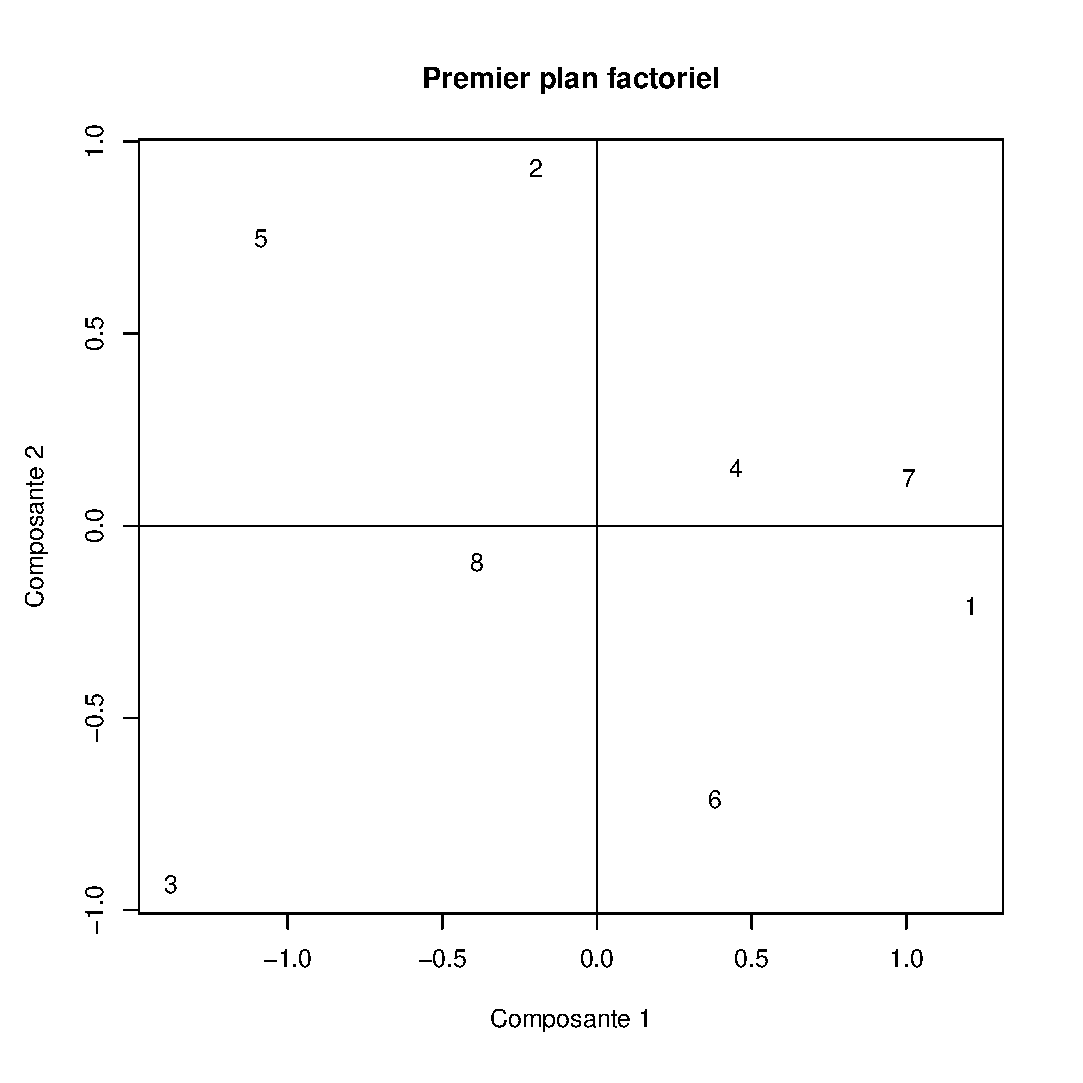
\includegraphics[width=6.5cm]{./img/q-5_premier_plan_fac.eps}
\includegraphics[width=6.5cm]{./img/q-5_second_plan_fac.eps}
\caption{Premier et second plan factoriel}
\label{q.5.premier_plan_fac}
\end{figure}

% \begin{figure}[H]
% \centering
% \includegraphics[width=9cm]{./img/q-5_second_plan_fac.eps}
% \caption{Second plan factoriel}
% \label{q.5.second_plan_fac}
% \end{figure}
%TO DO : à interpréter

Les individus du premier plan factoriel \ref{q.5.premier_plan_fac} sont situés d'une manière similaire au premier plan factoriel de la figure \ref{q.1.premier_plan_fac} sans les individus 8 et 2. Ici, l'axe 2 et 3 explique bien l'individu 2 alors que seul l'axe 3 explique bien l'individu 8.


%Utilisation des outils R
\subsection{Utilisation des outils R}
\subsubsection*{1. Retrouver tous les résultats avec princomp}
On obtient l'ACP avec la fonction : \textbf{corr.pr<-princomp(data)} qui retourne un objet et affiche l'écart type pour chaque composantes.

On obtient l'écart type des composantes principales (donc la racine des valeurs propres), la proportion de la variance et la proportion cumulée par : \textbf{summary(corr.pr)}

Les vecteurs propres ou axes factoriels sont accessibles par \textbf{corr.pr\$loadings}.

On obtient les coordonnées des individus par les composantes principales dans la variable \textbf{corr.pr\$scores}.

\textbf{plot(corr.pr)} affiche un histogramme des variances de chaque composante.

\textbf{biplot(corr.acp)} affiche sur le même graphique les individus et les variables sur le premier plan factoriel.

\textbf{biplot.princomp} est la fonction générale de \textbf{biplot}. Elle peut prendre plusieurs arguments : 
\begin{itemize}
	\item \textit{choices} : permet de choisir les axes principaux à représenter
    \item \textit{scale} : permet de mettre les données à l'échelle (entre 0 et 1)
\end{itemize}

Nous avons retrouvé les résultats obtenus en \ref{2.} avec ces fonctions.


\subsubsection*{2. Les resultats de princomp}

Avec la fonction plot, on obtient les variance exprimées par les composantes principales.
Avec la fonction biplot, on obtient la représentation des individus et des variables qui combine les représentations trouvées en [\ref{q.1.premier_plan_fac}] et [\ref{2.1.var_plot_fac}] (Les axes sont orientés dans le sens opposé).

\begin{figure}[H]
\centering
\includegraphics[width=5cm]{./img/princomp_1.png}
\includegraphics[width=5cm]{./img/princomp_2.png}
\caption{Le résultat des fonctions plot et biplot}
\end{figure}



%TO DO
%%%%%%%%%ACP Crabs
\subsection{Données Crabs}
Sans traitement préalable, on effectue un ACP sur les données. Les variances exprimées et la représentation du biplot sont présentées par les figures suivantes [\ref{2.3.var_acp}] :

\begin{figure}[H]
\centering
\includegraphics[width=5cm]{./img/acp_crabs_variance.png}
\includegraphics[width=5cm]{./img/acp_crabs_biplot.png}
\caption{Variances exprimées et la représentation des individus}
\label{2.3.var_acp}
\end{figure}

On observe que la première composante contient une très grande partie de l'information, car elle a une inertie expliquée de 98.2\%. (table \ref{2.3.tab_vp}), alors que la deuxième composante explique moins d'1\% de la variance totale.\\
Cela signifie que les individus varient très fortement selon une composante uniquement.
Comme nous l'avons expliqué en \ref{1.2.2}, les mensurations des crabes sont toutes corrélées car elles sont proportionnelles entre elles. La première composante est un indicateur de la taille et donc de la forme des crabes. De plus, la très faible variance de la deuxième composante confirme que les crabes restent proportionnels à leurs mensurations pour toutes les espèces et sexes car les individus sont uniquement expliqués par la première composante.


Toutes les variables du biplot \ref{2.3.var_acp} sont expliquées par la première composante mais très peu par la deuxième sauf pour RW qui est en plus légèrement expliquée par la deuxième composante. Cela est expliqué par le fait que les variables sont fortement corrélées comme nous l'avons vu en \ref{1.2.2}.\\
En particulier, on observe que les variables [CL,CW] ; [FL,BD] sont regroupées ensemble et que RW est proche de [FL,BD] mais quelque peu distante. Autrement dit, chaque groupe de variables exprime un attrait différent sur les individus. Cela explique que l'on ait pu identifier une bonne partie des espèces ou le sexe avec une combinaison de [CL ou CW] avec [FL ou BD] ou avec RW car ces caractéristiques ne sont pas regroupées ensemble.

De plus, il n'est pas possible d'identifier visuellement des groupes d'individus sur le biplot.

\begin{figure}[H]
\centering
\includegraphics[width=6.5cm]{./img/acp_crabs_classification_1.png}
\caption{Visualisation dans le premier plan factoriel}
\label{viz_sp_sex_pca}
\end{figure}

Avec de grandes variances exprimées par la première et la deuxième composante principale, on pouvait identifier des catégories, mais ce n'est pas le cas dans ce jeu de données. Nous n'avons pas une claire frontière entre l'espèce 'O' et 'B'. 

La figure nous montre que le sexe empêche la distinction des groupes. Dans le tableau de p-value (table \ref{table1.2.1}), on trouve une dépendance entre RW et sexe. Une solution est donc d'enlever la variable RW.

D'après la figure \ref{viz_sp_sex_pca}, on peut identifier le sexe sachant l'espèce de l'individu selon la deuxième composante principale. Il y a une certaine frontière entre les triangles et les cercles.

Aussi, comme la forme d'un crabe est proportionnelle à toutes ses mensurations chaque combinaison d'espèce et de sexe, une autre solution serait de diviser chaque mensuration par la taille totale de ses membres (donc la somme de ses mensurations). Nous effectuons ainsi une mise à l'échelle des individus.


\subsubsection*{2.}
Après avoir enlevé la variable RW, on reconduit une ACP. La visualisation est présentée par le diagramme suivant :

\begin{figure}[H]
\centering
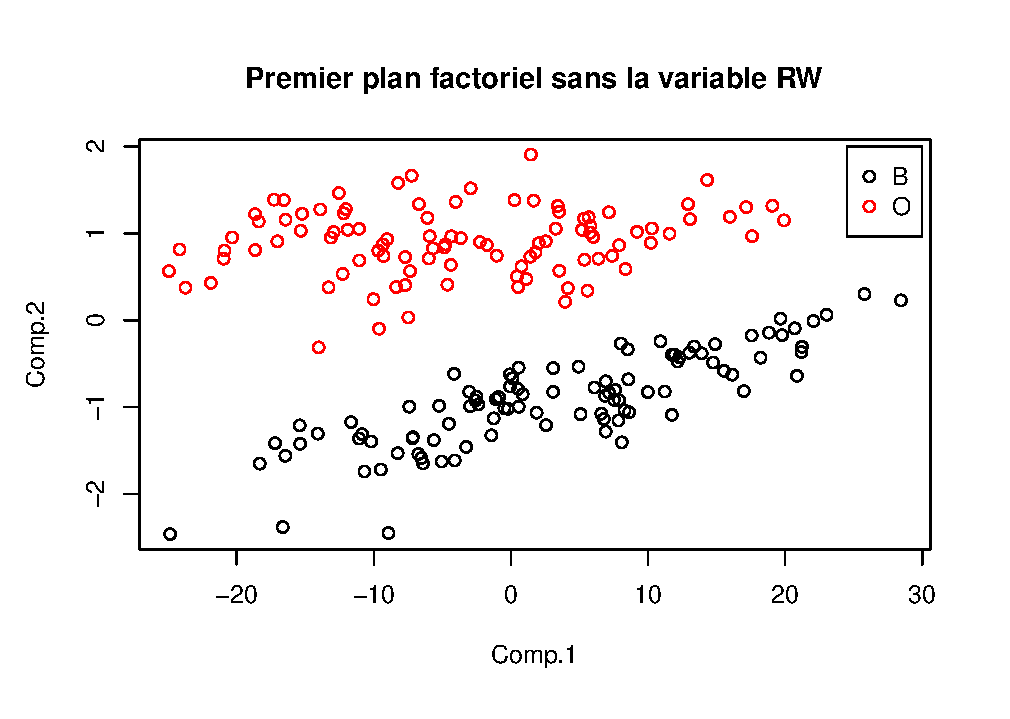
\includegraphics[width=7cm]{./img/2-3_premier_plan_no_rw.eps}
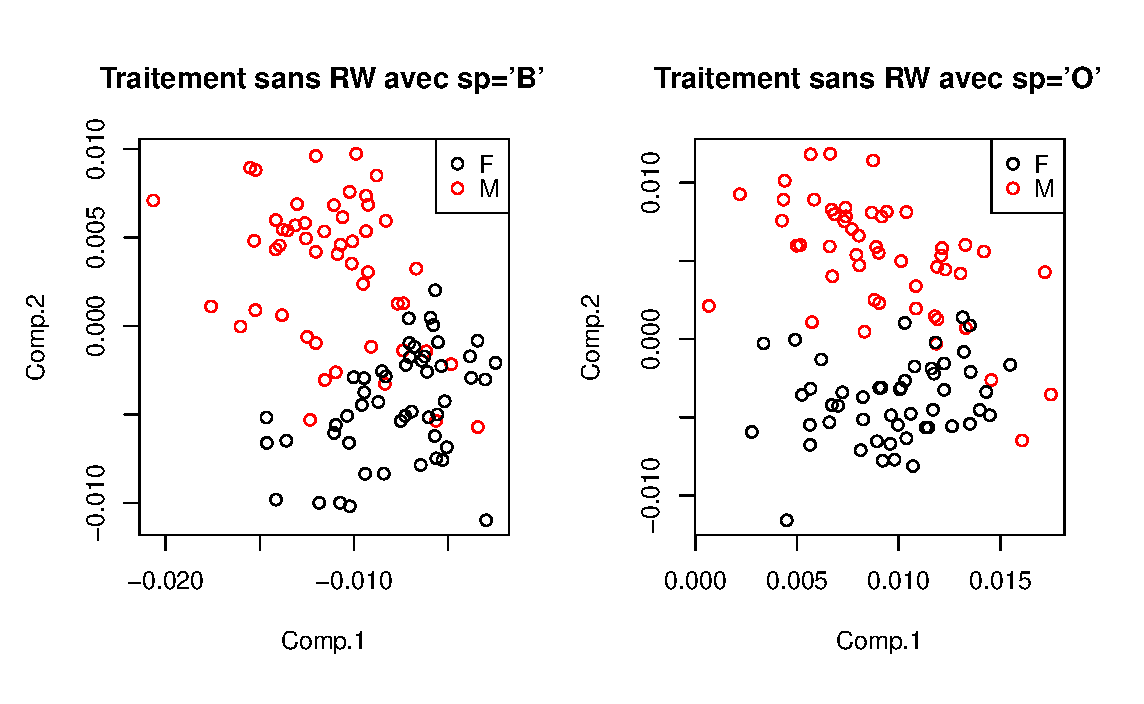
\includegraphics[width=7.5cm]{./img/2-3_premier_plan_no_rw_sp.eps}
\caption{Représentation des individus après avoir enlevé RW}
\label{viz_sp_sans_rw}
\end{figure}

La figure \ref{viz_sp_sans_rw} montre qu'il y a une frontière claire entre l'espèce 'B' et 'O' qui permet donc d'identifier ces individus. De plus, en connaissant l'espèce de l'individu, on a une frontière entre les différents sexes.

% \begin{figure}[H]
% \centering
% %\includegraphics[width=14cm]{./img/acp_crabs_final_sexe.png}
% 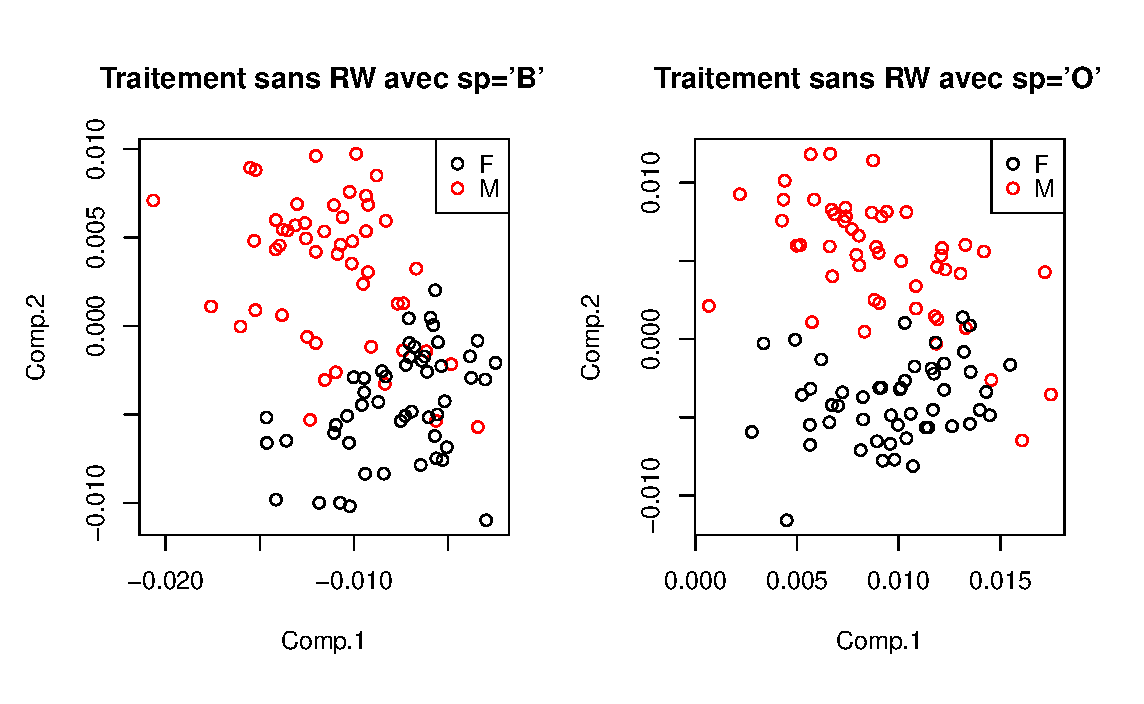
\includegraphics[width=7cm]{./img/2-3_premier_plan_no_rw_sp.eps}
% \caption{Représentation des individus dans le premier plan factoriel\\après avoir enlevé RW}
% \label{class_sp_sans_rw}
% \end{figure}


Avec la solution de mise à l'échelle, on obtient l'inertie expliquée suivante :

\begin{figure}[H]
\centering
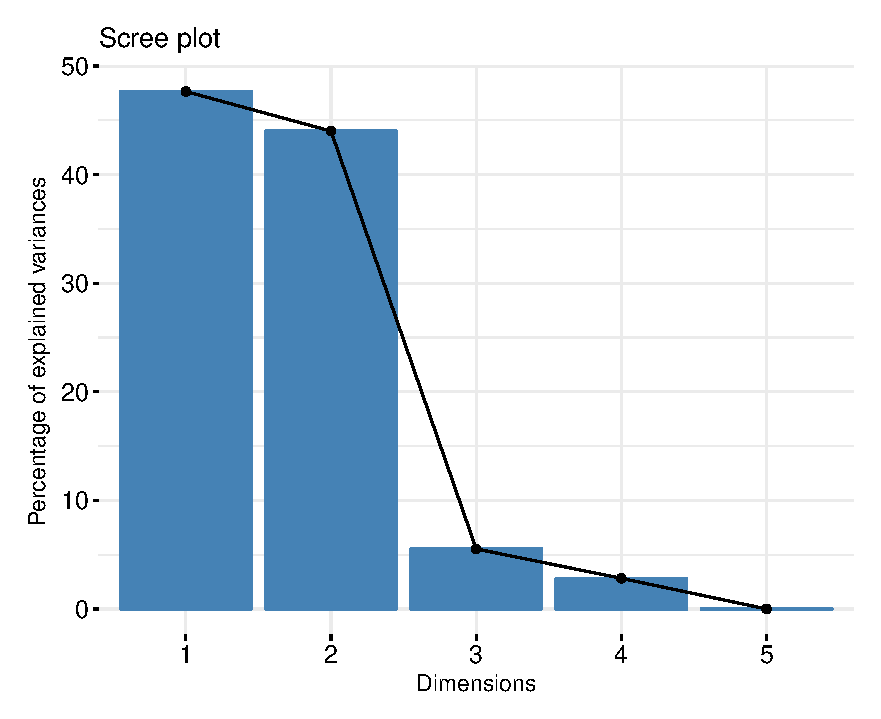
\includegraphics[width=4.5cm]{./img/2-3_screeplot_scaled.eps}
\caption{Inertie expliquée de l'ACP}
\label{2.3.screeplot_scaled}
\end{figure}
Dans ce cas, la variance de la première composante est bien distribuée à la deuxième et un peu à la troisième composante comparativement à [\ref{2.3.var_acp}].

Les individus sont représentés par les biplots suivants :
(species à gauche, sexe à droite).
\begin{figure}[H]
\centering
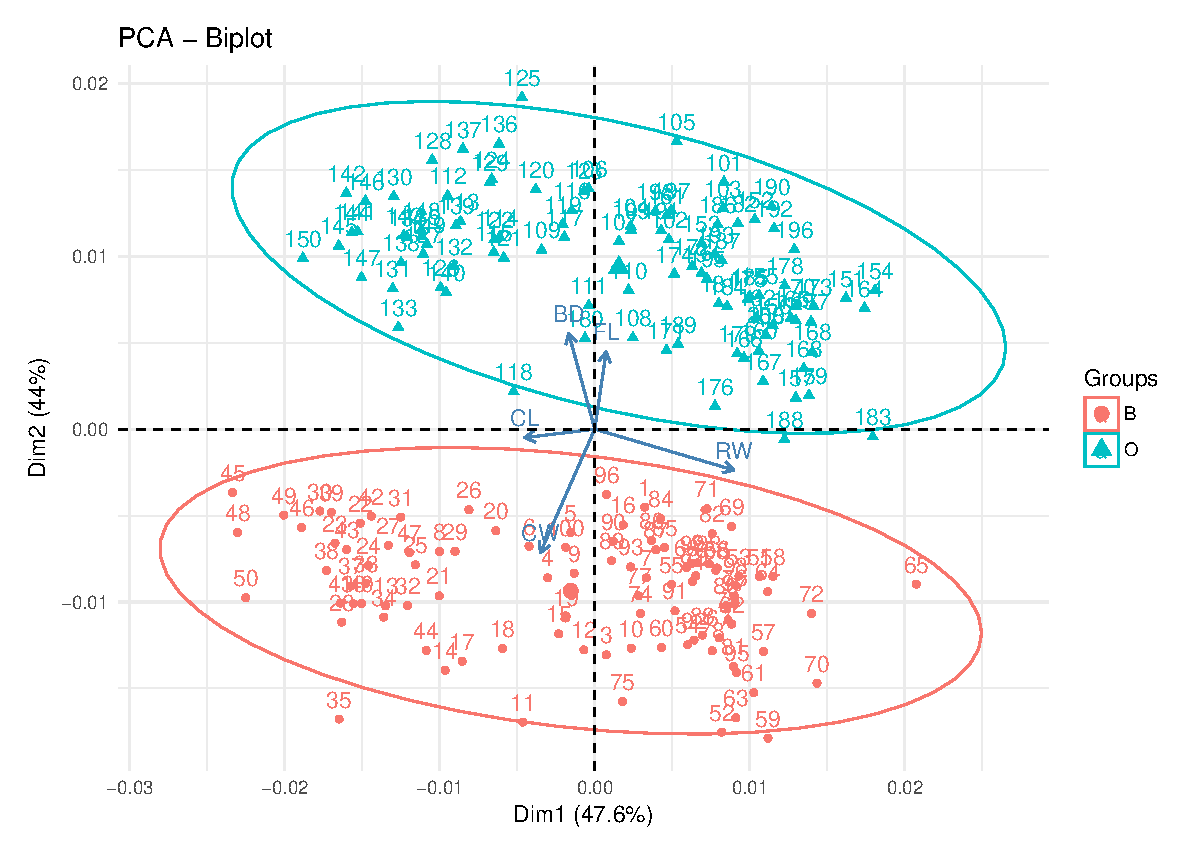
\includegraphics[width=7.5cm]{./img/2-3_biplot_pca_scaled_sp.eps}
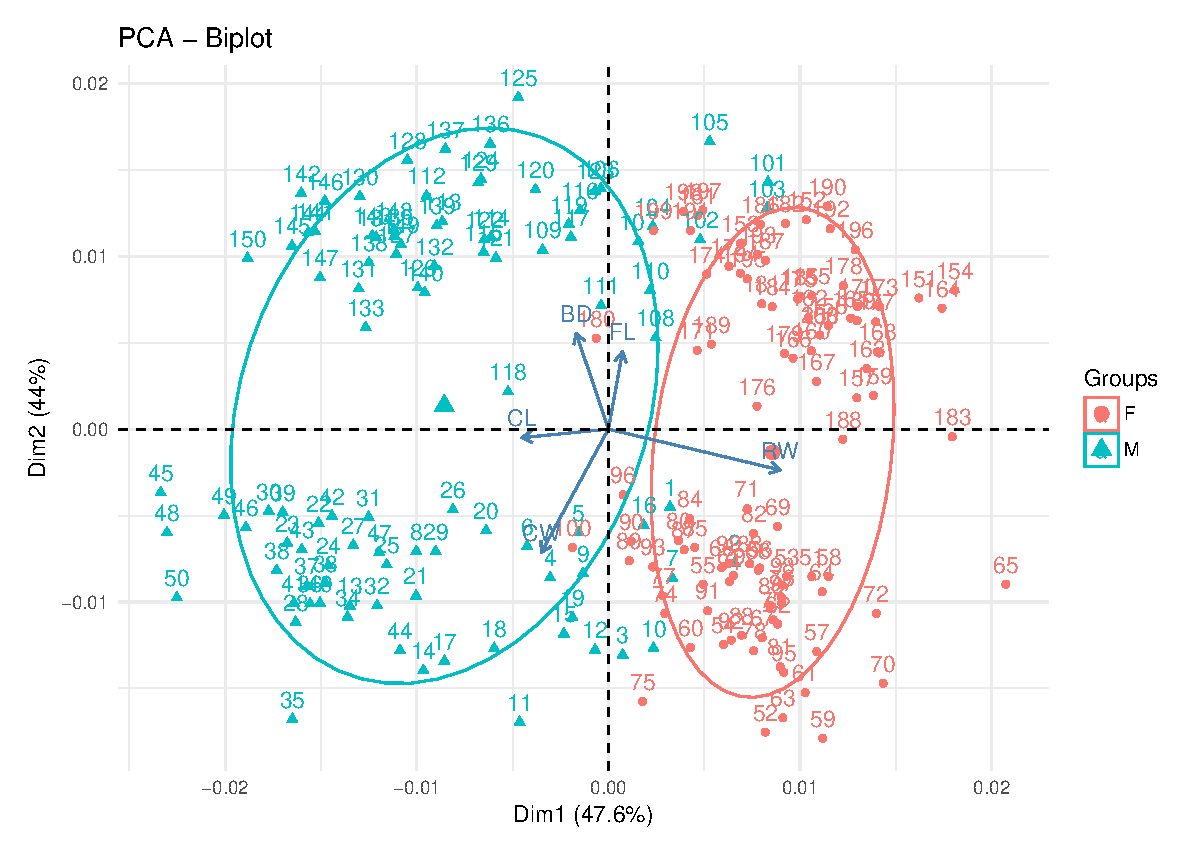
\includegraphics[width=7.5cm]{./img/2-3_biplot_pca_scaled_sex.eps}
\caption{Représentation des individus et variables dans le nouvel espace}
\label{2.3.biplot_scaled_sp}
\end{figure}

D'après la figure \ref{2.3.biplot_scaled_sp}, nous en déduisons que l'espèce est facilement discernable selon la composante 1 et 2. L'ellipse du biplot pour l'espèce est fixée de sorte à contenir les individus à taux de confiance de 95\%.

% \begin{figure}[H]
% \centering
% 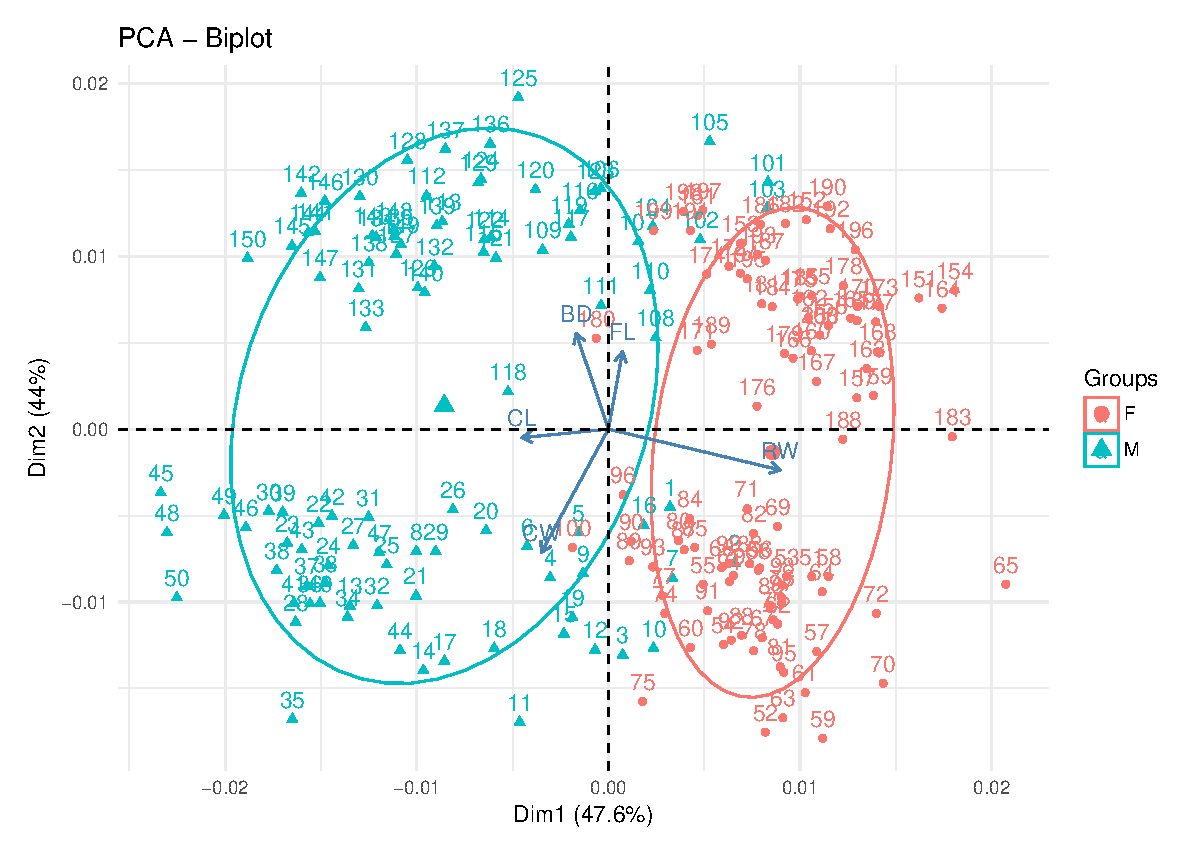
\includegraphics[width=11cm]{./img/2-3_biplot_pca_scaled_sex.eps}
% \caption{Représentation des individus et variables dans le nouvel espace}
% \label{2.3.biplot_scaled_sex}
% \end{figure}

De même, la figure \ref{2.3.biplot_scaled_sp} montre que le sexe est facilement identifiable par la composante 1 et 2 avec un recouvrement tout de même plus visible que pour le biplot du sexe. L'ellipse est paramétrée à un taux de 68\%. En fait, en combinant ces deux représentations, nous pouvons maintenant distinguer 4 groupes correspondant aux combinaisons de species et de sex.

On remarque que les variables représentées ne sont plus alignées dans la même direction : RW et CW sont presque orthogonaux.




%%%%%%%%%%ACP Pima
\subsection{Données Pima}
Nous avons effectué l'ACP sans traitement préalable et il semble difficile de distinguer visuellement les groupes dans le premier plan factoriel [\ref{acp_pima_2d}]. Par contre, on peut voir une frontière un peu plus claire sur la représentation des trois premiers axes principaux [\ref{acp_pima_3d}].

\begin{figure}[H]
\centering
\includegraphics[width=7cm]{./img/acp_pima.png}
\caption{Représentation des individus dans le premier plan factoriel\\(Diabétique : rouge, Non diabétique : noir)}
\label{acp_pima_2d}
\end{figure}

\begin{figure}[H]
\centering
\includegraphics[width=7cm]{./img/acp_pima_3d.png}
\caption{Représentation de pima dans 3 dimensions\\ (Diabétique : rouge, Non diabétique : noir)}
\label{acp_pima_3d}
\end{figure}

Les corrélations des variables dans la question \ref{1.3.2} montrent que les variables quantitatives sont assez indépendantes les unes des autres.\\
Les deux premières composantes principales (table \ref{Table2.4}) n'expriment pas assez d'information. Par conséquent, on a besoin de plus de dimensions pour pouvoir discerner les groupes d'individus.

Ainsi, comme nous l'avions pressenti en \ref{1.3.2}, il est dans ce cas difficile pour l'ACP de trouver des composantes principales réduisant assez le nombre de dimensions jusqu'à moins de 3 pour distinguer les deux catégories de patientes.

\section*{Conclusion}
%%%% TO DO

Ce TP nous a permis d'appliquer des concepts de base de statistiques afin d'avoir une première vue sur divers jeux de donnée tant au niveau du nombre de variables qu'au degré de corrélation entre-elles. Nous avons ensuite appliqué une ACP afin d'approfondir notre analyse sur ces jeux de données. Cela nous a permis d'identifier visuellement des groupes et constitue une première approche à l'apprentissage non supervisé.  


%\begin{thebibliography}{99} 
\section*{Références}
[1] \href{http://www.sthda.com/english/wiki/principal-component-analysis-in-r-prcomp-vs-princomp-r-software-and-data-mining}{Principal component analysis in R : prcomp() vs. princomp() - R software and data mining}

%\bibitem [1]{stock} \href{http://www.sthda.com/english/wiki/principal-component-analysis-in-r-prcomp-vs-princomp-r-software-and-data-mining}{Principal component analysis in R : prcomp() vs. princomp() - R software and data mining}


\section*{Annexes}

\begin{table}[H]
\caption{Descriptif statistique des variables quantitatives de \ref{1.1.1}}
\label{anx1}
\centering
\resizebox{7.5cm}{!}{%
\begin{tabular}{ l| c c c c c c c}

 & Min & 1st Qu. & Median & Moyenne & 3rd Qu. & Max & Std. dev.\\ 
\cline{1-3}
\hline
Note median & 0 & 8 & 11 & 10.92 & 14 & 20 & 3.82\\ 
Note final & 0 & 9.5 & 13 & 12.38 & 16 & 19.5 & 4.25 \\ 
Note total & 0.9 & 9.78 & 12.3 & 11.85 & 14.80 & 18.40 & 3.44\\

\end{tabular}
}
\end{table}


\begin{table}[!ht]
\caption{Tableau des p-value du test du Chi2 entre les variables qualitatives de \ref{1.1.1} et le \textit{resultat}\\pour l'hypothèse d'indépendance}
\label{anx6}
\centering
\resizebox{5.5cm}{!}{
\begin{tabular}{l|c|c}
%\hline
 & \multicolumn{2}{c}{resultat} \\
\hline
specialite&2.08e-2&Rejetée\\
%\hline
niveau&3.52e4-&Rejetée\\
%\hline
dernier diplome obtenu& 2.57e-1&Non rejetée\\
%\hline
correcteur median& 6.96e-1 &Non rejetée\\
%\hline
correcteur final& 7.31e-1 &Non rejetée\\
%\hline
\end{tabular}
}
\end{table}


\begin{table}[!ht]
\caption{Tableau des p-value du test de Student pour l'hypothèse d'indépendance entre le correcteur et l'examen corrigé (Examen médian à gauche, final à droite)}
\label{anx7}
%\centering
\resizebox{\columnwidth}{1.2cm}{
\begin{tabular}{l|ccccccc|c}

& Cor1 & Cor2 & Cor4 & Cor5 & Cor6 & Cor7 & Cor8 & Couple avec hypothèse rejetée\\
\hline
Cor1 & 1 & & & & & & & $\backslash$\\
Cor2 & 0.182 & 1 & & & & & &$\backslash$\\
Cor4 & 0.605 & 0.0117 & 1 & & & & & $\backslash$\\
Cor5 & 0.790 & 0.216 & 0.333 & 1 & & && $\backslash$\\
Cor6 & 0.435 & 0.533 & 0.096 & 0.556 & 1 & && $\backslash$\\
Cor7 & 0.554 & 0.018 & 0.878 & 0.312 & 0.105 & 1 & &$\backslash$\\
Cor8 & 0.979 & 0.243 & 0.625 & 0.832 & 0.499 & 0.575 & 1 &$\backslash$\\

\end{tabular}

\begin{tabular}{l|ccccccc|c}

&Cor1 & Cor3 & Cor4 & Cor5 & Cor6 & Cor7 & Cor8 & Couple avec hypothèse rejetée\\
\hline
Cor1 & 1 & & & & & & &$\backslash$\\
Cor3 & 0.130 & 1 & & & & & & $\backslash$\\
Cor4 & 0.030 & 0.301 & 1 & & & & &(Cor4, Cor1)\\
Cor5 & 0.416 & 0.345 & 0.066 & 1 & & &&$\backslash$ \\
Cor6 & 0.038 & 0.344 & 0.984 & 0.088 & 1 & &&(Cor6, Cor1) \\
Cor7 & 0.395 & 0.426 & 0.097 & 0.932 & 0.120 & 1 && $\backslash$\\
Cor8 & 0.738 & 0.302 & 0.092 & 0.708 & 0.105 & 0.671 & 1&$\backslash$ \\

\end{tabular}
}
\end{table}


\begin{table}[H]
\caption{Tableau de corrélation des variables quantitatives de \ref{1.1.1}}
\label{anx5}
\centering
\resizebox{6.1cm}{!}{
\begin{tabular}{ l| c c c}

 & Note median & Note final & Note totale\\ 
\hline
Note median & 1 & & \\ 
Note final & 0.386 & 1 & \\ 
Note total & 0.730 & 0.912 & 1\\

\end{tabular}
}
\end{table}





%%%%%%%%%% 1.2


\begin{table}[H]
\caption{Descriptif statistique des variables quantitatives de \ref{1.2.1}}
\label{anx2.1}
\centering
\resizebox{7cm}{!}{%
\begin{tabular}{ l| c c c c c c c}

 & Min & 1st Qu. & Median & Moyenne & 3rd Qu. & Max & Std. dev.\\ 
\cline{1-3}
\hline
FL & 7.20 & 12.90 & 15.55 & 15.58 & 18.05& 23.10 & 3.50 \\ 
RW & 6.5 & 11.00 & 12.80 & 12.74 & 14.30 & 20.20  & 2.57\\ 
CL & 14.70 & 27.27 & 32.10 & 32.11 & 37.23 & 47.60 & 7.12\\
CW & 17.1 & 31.50 & 36.80 & 36.41 & 42.00 & 54.60 & 7.87\\
BD & 6.1 & 11.40 & 13.90 & 14.03 & 16.60 & 21.60 & 3.42\\


\end{tabular}
}
\end{table}


\begin{table}[!h]
\centering
\caption{Tableau des p-value du test de Student entre les variables quantitatives et qualitatives de \ref{1.2.1}}\label{table1.2.1}
\label{Table2.1}
\resizebox{6.5cm}{!}{
\begin{tabular}{l|c|c|c|c}

 & \multicolumn{2}{c}{Espèce} &\multicolumn{2}{|c}{Sexe} \\
\hline
FL& 8.970e-11&Dépendant& 5.426e-01&Indépendant\\
%\hline
RW& 5.306e-06&Dépendant & 2.862e-05&Dépendant\\
%\hline
CL& 3.468e-05&Dépendant & 1.390e-01&Indépendant\\
%\hline
CW& 2.109e-03 &Dépendant& 2.949e-01&Indépendant\\
%\hline
BD& 4.065e-10 &Dépendant& 2.064e-01&Indépendant\\

\end{tabular}
}
\end{table}


% \begin{figure}[!ht]
% \centering
% 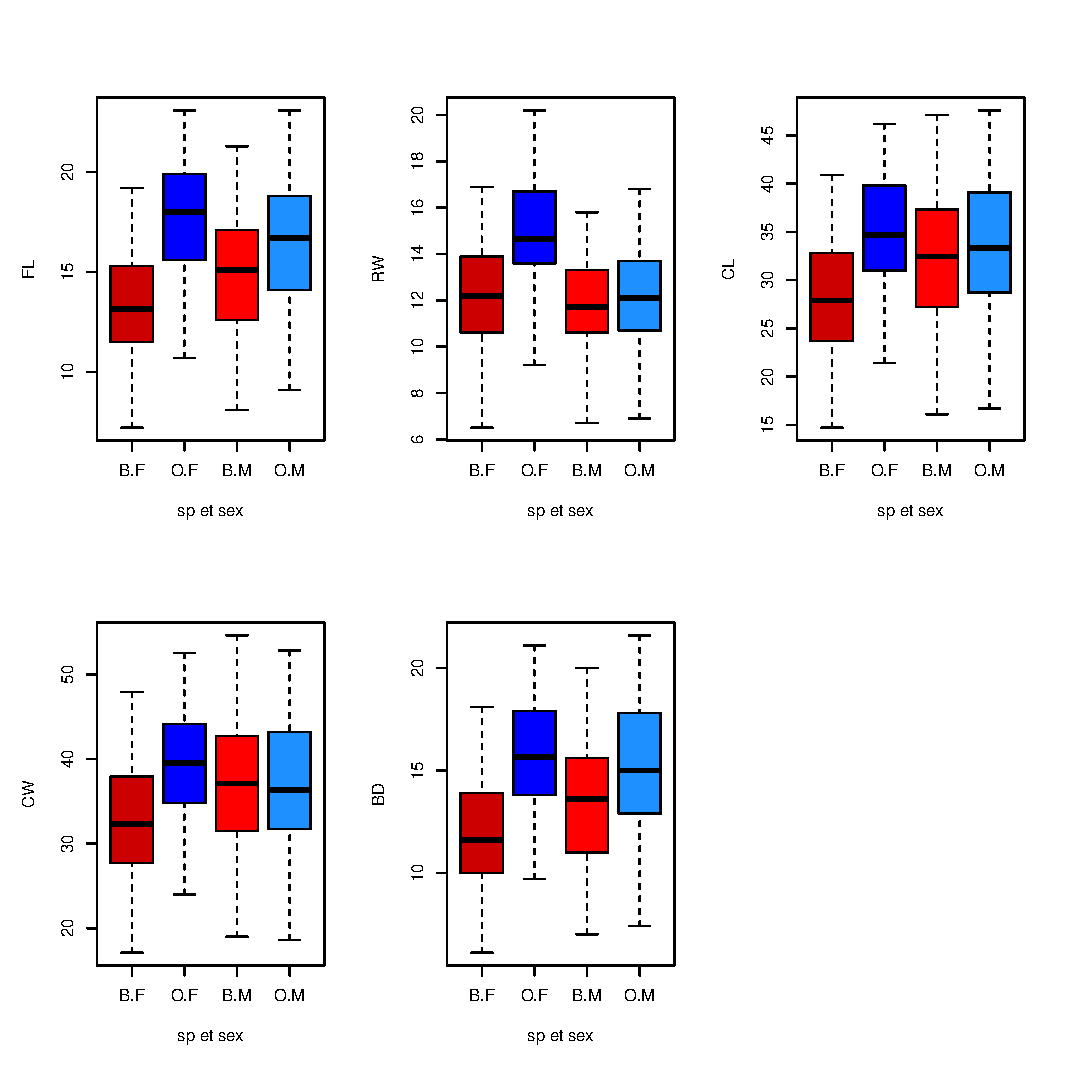
\includegraphics[width=7.6cm]{./img/1-2-boxplot_sp_sex.eps}
% \caption{Diagramme en boîte de la morphologie en fonction de l'espèce et du sexe}
% \label{fig:sp_sex_ssp_morphologique}
% \end{figure}


\begin{table}[!ht]
\centering
\caption{Corrélation entre les caractériques morphologiques}\label{table1.2.2}
\resizebox{4.5cm}{!}{%
\begin{tabular}{c|ccccc}

 &FL&RW&CL&CW&BD\\
\hline
FL& 1&&&&\\

RW& 0.907&1 & &&\\

CL& 0.979&0.893&1 &&\\

CW& 0.965&0.900& 0.995&1&\\

BD&0.988&0.889&0.983&0.968&1\\

\end{tabular}
}
\end{table}


\begin{figure}[!h]
\centering
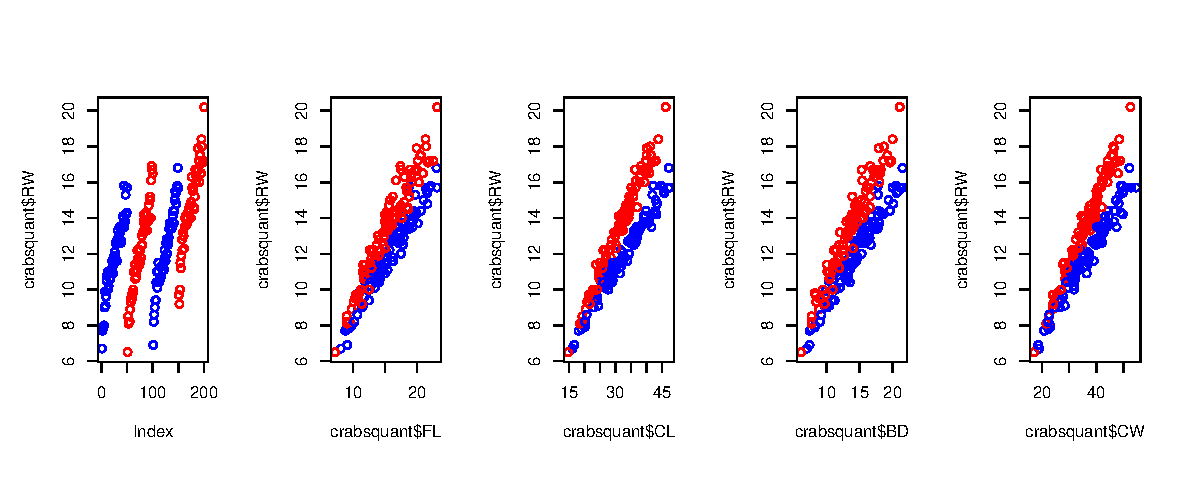
\includegraphics[width=11cm]{./img/1-2-pairs_identif_sex.eps}
\caption{Représentation des individus en fonction du sexe ('F' : rouge, 'M' : Bleu) par l'index et les variables quantitatives identifiants fortement l'espèce}
\label{fig:pairs-plot_identif_sex}
\end{figure}



%%%%%%%% 1.3


\begin{table}[H]
\caption{Descriptif statistique des variables quantitatives de \ref{1.3.1}}
\label{anx3.1}
\centering
\resizebox{8cm}{!}{%
\begin{tabular}{ l| c c c c c c c}

 & Min & 1st Qu. & Median & Moyenne & 3rd Qu. & Max & Std. dev.\\ 
\cline{1-3}
\hline
npreg & 0 & 1 & 2 & 3.52 & 5& 17 & 3.31 \\ 
glu & 56 & 98.75 & 115 & 121.03 & 141.25 & 199  & 31\\ 
bp & 24 & 64& 72& 71.51 & 80 & 110 &12.31 \\
skin & 7 & 22 & 29 & 29.18 & 36 & 99 & 10.52\\
bmi & 18.20 & 27.88 & 32.80 & 32.89 & 36.90 & 67.10 & 6.88\\
ped&0.09&0.26&0.42&0.50&0.66&2.42&0.34\\
age & 21 &23 &28 &31.61 &38 &81 &10.76\\


\end{tabular}
}
\end{table}


\begin{table}[!ht]
\centering
\caption{Corrélation entre les variables quantitatives}\label{table1.3.1}
\resizebox{6.5cm}{!}{%
\begin{tabular}{c|ccccccc}

&npreg & glu & bp & skin & bmi & ped & age\\
\hline
npreg & 1 & & & & &  \\
glu & 0.125 & 1 & & & &  \\
bp & 0.205 & 0.219 & 1 & & &  \\
skin & 0.095 & 0.227 & 0.226 & 1 & &  \\
bmi & 0.009 & 0.247 & 0.307 & 0.647 & 1 &  \\
ped & 0.007 & 0.166 & 0.008 & 0.119 & 0.151 & 1 \\
age & 0.641 & 0.279 & 0.347 & 0.161 & 0.073 & 0.072 & 1

\end{tabular}
}
\end{table}


\begin{table}[!ht]
\caption{Tableau des p-value du test de Student en fonction du facteur diabète}
\centering

\resizebox{4.3cm}{!}{%
\begin{tabular}{l|c|c}

 & \multicolumn{2}{c}{Résultat du test de Student}\\
\hline
npreg  &1.617e-07&dépendant\\
glu &2.362e-28&dépendant\\
bp &3.103e-05&dépendant\\
skin &4.862e-09&dépendant\\
bmi &2.887e-12&dépendant\\
ped & 9.266e-07&dépendant\\
age &1.055e-12&dépendant\\
\end{tabular}
}

\label{table1.3_student}
\end{table}


%%%%%%%%%%% PArtie 2


%%%% 2.1.5

\begin{figure}[!ht]
\centering
\begin{adjustbox}{width=12cm,height=0.7cm,keepaspectratio}
\begin{lstlisting}{language=R}
for(i in 1:ncol(corr.acp)){
  corr.acp[is.na(corr.acp[,i]), i] <- mean(corr.acp[,i], na.rm = TRUE)
}
\end{lstlisting}
\end{adjustbox}
\caption{Code R pour remplacer des valeurs manquantes par la moyenne des colonnes}
\label{code_R_na}
\end{figure}



\begin{table}[H]
\caption{Valeurs propres et inertie expliquée par les axes factoriels [\ref{2.1.5}]}
\label{2.1.5tab_vp}
\centering

\resizebox{7.4cm}{!}{%
\begin{tabular}{l|c|c|c|c}

& $\lambda_{1}$ & $\lambda_{2}$ & $\lambda_{3}$ & $\lambda_{4}$\\
\hline
Valeur	& 0.761 & 0.362 & 0.162 & 0.120\\
Inertie expliquée (\%) & 54.2 & 25.8 & 11.5 & 8.50\\
Inertie expliquée cumulée (\%) ($E_{k}$) & 54.2 & 79.9  & 91.5 & 100.0\\

\end{tabular}
}

\end{table}





%%%%%%% 2.3
\begin{table}[H]
\caption{Valeurs propres et inertie expliquée par les axes factoriels}
\centering
\resizebox{8cm}{!}{%
\begin{tabular}{l|c|c|c|c|c}

& $\lambda_{1}$ & $\lambda_{2}$ & $\lambda_{3}$ & $\lambda_{4}$ & $\lambda_{5}$\\
\hline
Valeur	& 140.00 & 1.29 & 1.00 & 0.13 & 0.078\\
Inertie expliquée (\%) & 98.2 & 0.91 & 0.70 & 0.09 & 0.05 \\
Inertie expliquée cumulée (\%) ($E_{k}$) & 98.2 & 99.2 & 99.95112 & 100.0 & 100.0\\

\end{tabular}
}

\label{2.3.tab_vp}
\end{table}


%%%%%%%%%%%% 2.4 


\begin{table}[H]
\centering
\caption{Inertie expliquée par les composantes principales}\label{table 2.4}
\label{Table2.4}
\resizebox{11cm}{!}{%
\begin{tabular}{|c|c|c|c|c|c|c|c|}
\hline
 &Comp.1&Comp.2&Comp.3&Comp.4&Comp.5&Comp.6&Comp.7\\
\hline
Standard deviation& 31.4579&13.4357& 10.6186&9.2122&4.5690&2.4770&3.358e-01\\
\hline
Proportion of Variance& 0.7094&0.1294 & 0.0808&0.0608&0.0149&0.0043&8.086e-05\\
\hline
Cumulative Proportion& 0.7095&0.8389&0.9197 &0.9806&0.9955&0.99991&1.0000\\
\hline
\end{tabular}
}
\end{table}





%\end{thebibliography}


%----------------------------------------------------------------------------------------
%\end{multicols}
\end{document}
